\documentclass[tikz]{standalone}
\usetikzlibrary{trees}
\begin{document}
\tikzstyle{every node}=[shape=rectangle,rounded corners,draw=black,thick,top color=white,bottom color=blue!20,anchor=west]
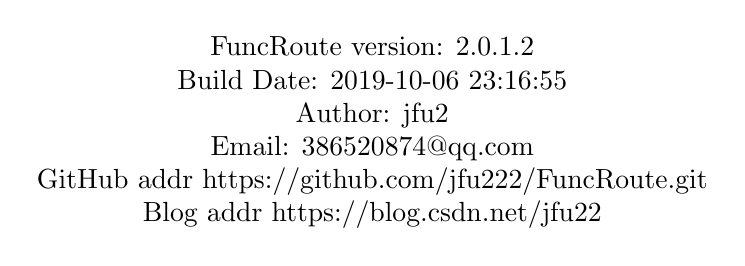
\begin{tikzpicture}
\node [align=center] {FuncRoute version: 2.0.1.2\\Build Date: 2019-10-06 23:16:55\\Author: jfu2\\Email: 386520874@qq.com\\GitHub addr https://github.com/jfu222/FuncRoute.git\\Blog addr https://blog.csdn.net/jfu22};
\end{tikzpicture}
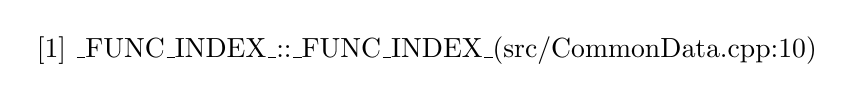
\begin{tikzpicture}[grow via three points={one child at (0.5,-0.7) and two children at (0.5,-0.7) and (0.5,-1.4)}, edge from parent path={(\tikzparentnode.south) |- (\tikzchildnode.west)}]
\node {[1] \_FUNC\_INDEX\_::\_FUNC\_INDEX\_(src/CommonData.cpp:10)}
;
\end{tikzpicture}

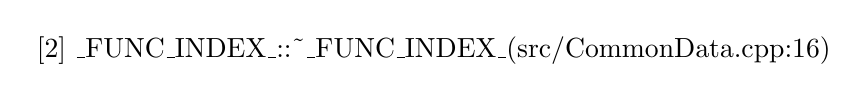
\begin{tikzpicture}[grow via three points={one child at (0.5,-0.7) and two children at (0.5,-0.7) and (0.5,-1.4)}, edge from parent path={(\tikzparentnode.south) |- (\tikzchildnode.west)}]
\node {[2] \_FUNC\_INDEX\_::\~{}\_FUNC\_INDEX\_(src/CommonData.cpp:16)}
;
\end{tikzpicture}

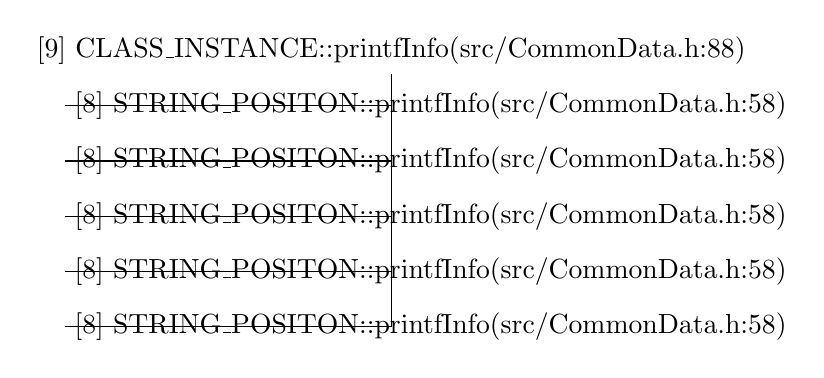
\begin{tikzpicture}[grow via three points={one child at (0.5,-0.7) and two children at (0.5,-0.7) and (0.5,-1.4)}, edge from parent path={(\tikzparentnode.south) |- (\tikzchildnode.west)}]
\node {[9] CLASS\_INSTANCE::printfInfo(src/CommonData.h:88)}
    child { node {[8] STRING\_POSITON::printfInfo(src/CommonData.h:58)} 
        }
    child { node {[8] STRING\_POSITON::printfInfo(src/CommonData.h:58)} 
        }
    child { node {[8] STRING\_POSITON::printfInfo(src/CommonData.h:58)} 
        }
    child { node {[8] STRING\_POSITON::printfInfo(src/CommonData.h:58)} 
        }
    child { node {[8] STRING\_POSITON::printfInfo(src/CommonData.h:58)} 
        }
;
\end{tikzpicture}

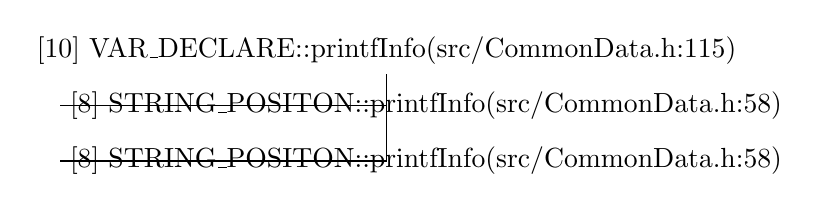
\begin{tikzpicture}[grow via three points={one child at (0.5,-0.7) and two children at (0.5,-0.7) and (0.5,-1.4)}, edge from parent path={(\tikzparentnode.south) |- (\tikzchildnode.west)}]
\node {[10] VAR\_DECLARE::printfInfo(src/CommonData.h:115)}
    child { node {[8] STRING\_POSITON::printfInfo(src/CommonData.h:58)} 
        }
    child { node {[8] STRING\_POSITON::printfInfo(src/CommonData.h:58)} 
        }
;
\end{tikzpicture}

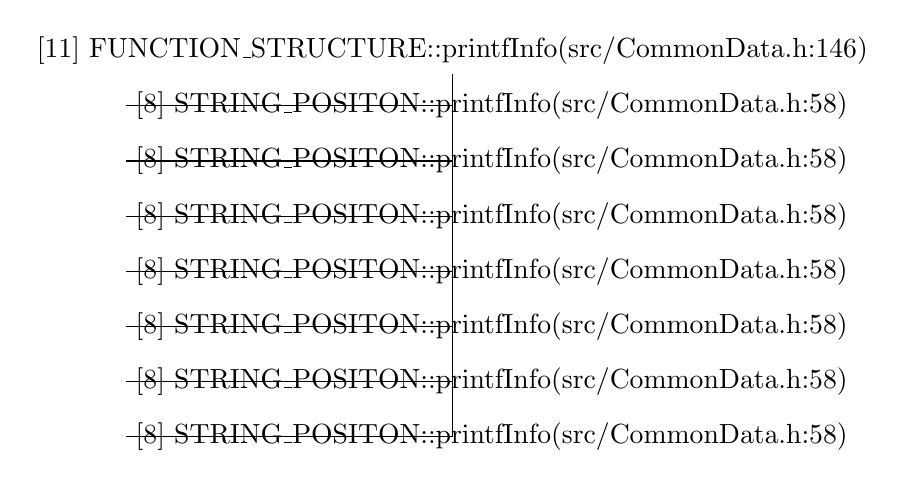
\begin{tikzpicture}[grow via three points={one child at (0.5,-0.7) and two children at (0.5,-0.7) and (0.5,-1.4)}, edge from parent path={(\tikzparentnode.south) |- (\tikzchildnode.west)}]
\node {[11] FUNCTION\_STRUCTURE::printfInfo(src/CommonData.h:146)}
    child { node {[8] STRING\_POSITON::printfInfo(src/CommonData.h:58)} 
        }
    child { node {[8] STRING\_POSITON::printfInfo(src/CommonData.h:58)} 
        }
    child { node {[8] STRING\_POSITON::printfInfo(src/CommonData.h:58)} 
        }
    child { node {[8] STRING\_POSITON::printfInfo(src/CommonData.h:58)} 
        }
    child { node {[8] STRING\_POSITON::printfInfo(src/CommonData.h:58)} 
        }
    child { node {[8] STRING\_POSITON::printfInfo(src/CommonData.h:58)} 
        }
    child { node {[8] STRING\_POSITON::printfInfo(src/CommonData.h:58)} 
        }
;
\end{tikzpicture}

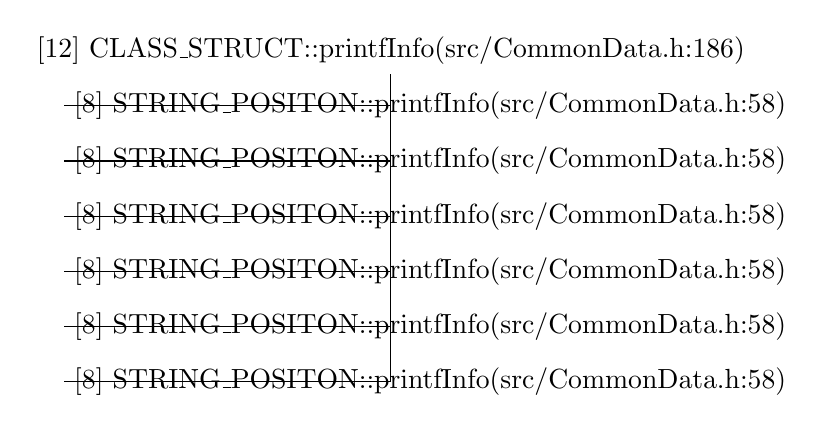
\begin{tikzpicture}[grow via three points={one child at (0.5,-0.7) and two children at (0.5,-0.7) and (0.5,-1.4)}, edge from parent path={(\tikzparentnode.south) |- (\tikzchildnode.west)}]
\node {[12] CLASS\_STRUCT::printfInfo(src/CommonData.h:186)}
    child { node {[8] STRING\_POSITON::printfInfo(src/CommonData.h:58)} 
        }
    child { node {[8] STRING\_POSITON::printfInfo(src/CommonData.h:58)} 
        }
    child { node {[8] STRING\_POSITON::printfInfo(src/CommonData.h:58)} 
        }
    child { node {[8] STRING\_POSITON::printfInfo(src/CommonData.h:58)} 
        }
    child { node {[8] STRING\_POSITON::printfInfo(src/CommonData.h:58)} 
        }
    child { node {[8] STRING\_POSITON::printfInfo(src/CommonData.h:58)} 
        }
;
\end{tikzpicture}

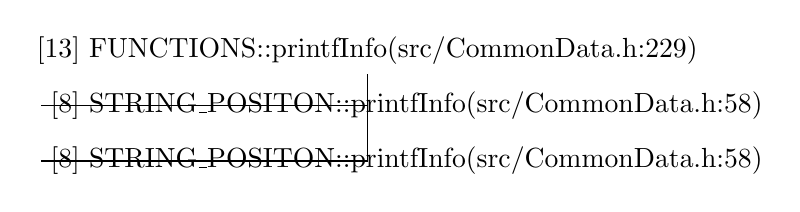
\begin{tikzpicture}[grow via three points={one child at (0.5,-0.7) and two children at (0.5,-0.7) and (0.5,-1.4)}, edge from parent path={(\tikzparentnode.south) |- (\tikzchildnode.west)}]
\node {[13] FUNCTIONS::printfInfo(src/CommonData.h:229)}
    child { node {[8] STRING\_POSITON::printfInfo(src/CommonData.h:58)} 
        }
    child { node {[8] STRING\_POSITON::printfInfo(src/CommonData.h:58)} 
        }
;
\end{tikzpicture}

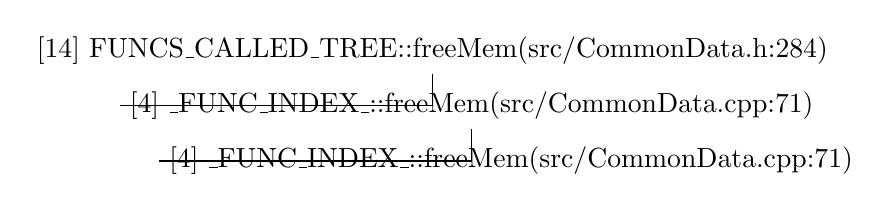
\begin{tikzpicture}[grow via three points={one child at (0.5,-0.7) and two children at (0.5,-0.7) and (0.5,-1.4)}, edge from parent path={(\tikzparentnode.south) |- (\tikzchildnode.west)}]
\node {[14] FUNCS\_CALLED\_TREE::freeMem(src/CommonData.h:284)}
    child { node {[4] \_FUNC\_INDEX\_::freeMem(src/CommonData.cpp:71)} 
        child { node {[4] \_FUNC\_INDEX\_::freeMem(src/CommonData.cpp:71)} 
            }
        }
        child [missing] {}
;
\end{tikzpicture}

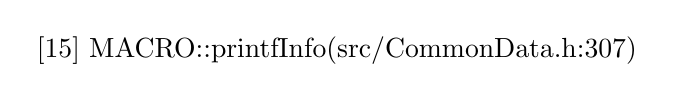
\begin{tikzpicture}[grow via three points={one child at (0.5,-0.7) and two children at (0.5,-0.7) and (0.5,-1.4)}, edge from parent path={(\tikzparentnode.south) |- (\tikzchildnode.west)}]
\node {[15] MACRO::printfInfo(src/CommonData.h:307)}
;
\end{tikzpicture}

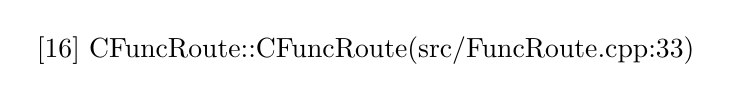
\begin{tikzpicture}[grow via three points={one child at (0.5,-0.7) and two children at (0.5,-0.7) and (0.5,-1.4)}, edge from parent path={(\tikzparentnode.south) |- (\tikzchildnode.west)}]
\node {[16] CFuncRoute::CFuncRoute(src/FuncRoute.cpp:33)}
;
\end{tikzpicture}

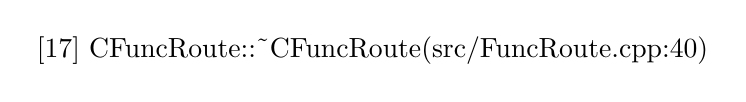
\begin{tikzpicture}[grow via three points={one child at (0.5,-0.7) and two children at (0.5,-0.7) and (0.5,-1.4)}, edge from parent path={(\tikzparentnode.south) |- (\tikzchildnode.west)}]
\node {[17] CFuncRoute::\~{}CFuncRoute(src/FuncRoute.cpp:40)}
;
\end{tikzpicture}

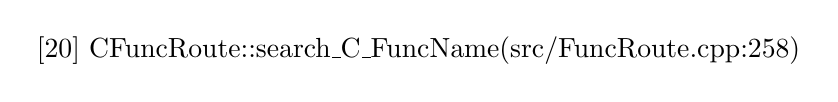
\begin{tikzpicture}[grow via three points={one child at (0.5,-0.7) and two children at (0.5,-0.7) and (0.5,-1.4)}, edge from parent path={(\tikzparentnode.south) |- (\tikzchildnode.west)}]
\node {[20] CFuncRoute::search\_C\_FuncName(src/FuncRoute.cpp:258)}
;
\end{tikzpicture}

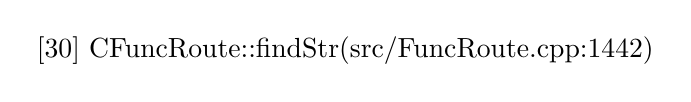
\begin{tikzpicture}[grow via three points={one child at (0.5,-0.7) and two children at (0.5,-0.7) and (0.5,-1.4)}, edge from parent path={(\tikzparentnode.south) |- (\tikzchildnode.west)}]
\node {[30] CFuncRoute::findStr(src/FuncRoute.cpp:1442)}
;
\end{tikzpicture}

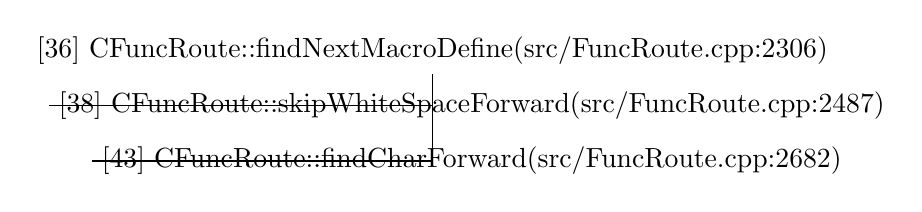
\begin{tikzpicture}[grow via three points={one child at (0.5,-0.7) and two children at (0.5,-0.7) and (0.5,-1.4)}, edge from parent path={(\tikzparentnode.south) |- (\tikzchildnode.west)}]
\node {[36] CFuncRoute::findNextMacroDefine(src/FuncRoute.cpp:2306)}
    child { node {[38] CFuncRoute::skipWhiteSpaceForward(src/FuncRoute.cpp:2487)} 
        }
    child { node {[43] CFuncRoute::findCharForward(src/FuncRoute.cpp:2682)} 
        }
;
\end{tikzpicture}

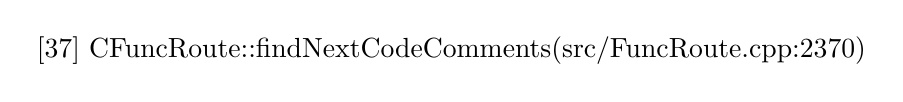
\begin{tikzpicture}[grow via three points={one child at (0.5,-0.7) and two children at (0.5,-0.7) and (0.5,-1.4)}, edge from parent path={(\tikzparentnode.south) |- (\tikzchildnode.west)}]
\node {[37] CFuncRoute::findNextCodeComments(src/FuncRoute.cpp:2370)}
;
\end{tikzpicture}

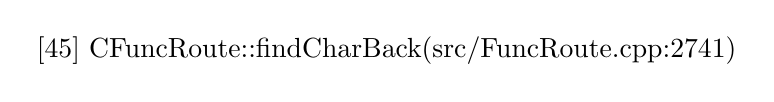
\begin{tikzpicture}[grow via three points={one child at (0.5,-0.7) and two children at (0.5,-0.7) and (0.5,-1.4)}, edge from parent path={(\tikzparentnode.south) |- (\tikzchildnode.west)}]
\node {[45] CFuncRoute::findCharBack(src/FuncRoute.cpp:2741)}
;
\end{tikzpicture}

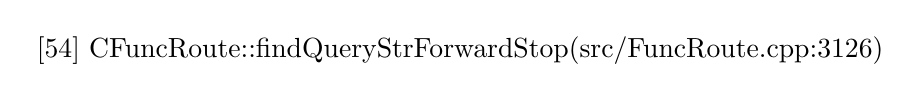
\begin{tikzpicture}[grow via three points={one child at (0.5,-0.7) and two children at (0.5,-0.7) and (0.5,-1.4)}, edge from parent path={(\tikzparentnode.south) |- (\tikzchildnode.west)}]
\node {[54] CFuncRoute::findQueryStrForwardStop(src/FuncRoute.cpp:3126)}
;
\end{tikzpicture}

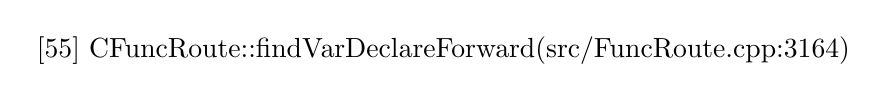
\begin{tikzpicture}[grow via three points={one child at (0.5,-0.7) and two children at (0.5,-0.7) and (0.5,-1.4)}, edge from parent path={(\tikzparentnode.south) |- (\tikzchildnode.west)}]
\node {[55] CFuncRoute::findVarDeclareForward(src/FuncRoute.cpp:3164)}
;
\end{tikzpicture}

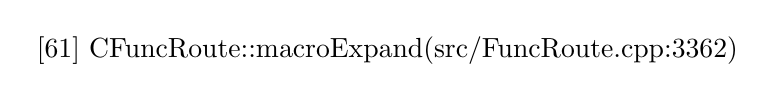
\begin{tikzpicture}[grow via three points={one child at (0.5,-0.7) and two children at (0.5,-0.7) and (0.5,-1.4)}, edge from parent path={(\tikzparentnode.south) |- (\tikzchildnode.west)}]
\node {[61] CFuncRoute::macroExpand(src/FuncRoute.cpp:3362)}
;
\end{tikzpicture}

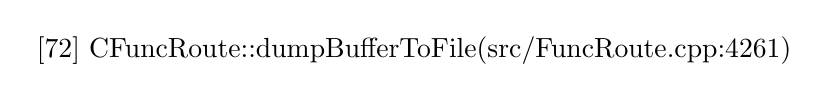
\begin{tikzpicture}[grow via three points={one child at (0.5,-0.7) and two children at (0.5,-0.7) and (0.5,-1.4)}, edge from parent path={(\tikzparentnode.south) |- (\tikzchildnode.west)}]
\node {[72] CFuncRoute::dumpBufferToFile(src/FuncRoute.cpp:4261)}
;
\end{tikzpicture}

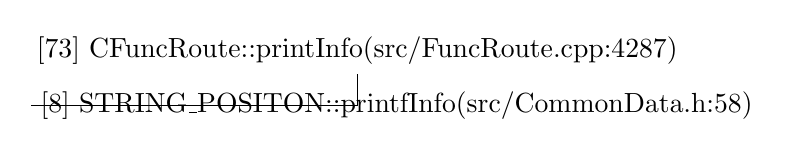
\begin{tikzpicture}[grow via three points={one child at (0.5,-0.7) and two children at (0.5,-0.7) and (0.5,-1.4)}, edge from parent path={(\tikzparentnode.south) |- (\tikzchildnode.west)}]
\node {[73] CFuncRoute::printInfo(src/FuncRoute.cpp:4287)}
    child { node {[8] STRING\_POSITON::printfInfo(src/CommonData.h:58)} 
        }
;
\end{tikzpicture}

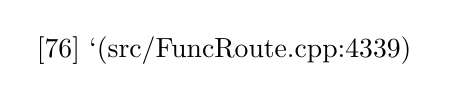
\begin{tikzpicture}[grow via three points={one child at (0.5,-0.7) and two children at (0.5,-0.7) and (0.5,-1.4)}, edge from parent path={(\tikzparentnode.south) |- (\tikzchildnode.west)}]
\node {[76] `(src/FuncRoute.cpp:4339)}
;
\end{tikzpicture}

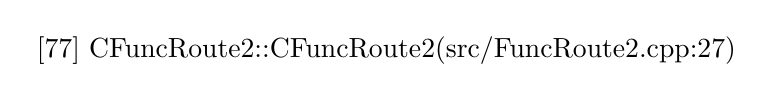
\begin{tikzpicture}[grow via three points={one child at (0.5,-0.7) and two children at (0.5,-0.7) and (0.5,-1.4)}, edge from parent path={(\tikzparentnode.south) |- (\tikzchildnode.west)}]
\node {[77] CFuncRoute2::CFuncRoute2(src/FuncRoute2.cpp:27)}
;
\end{tikzpicture}

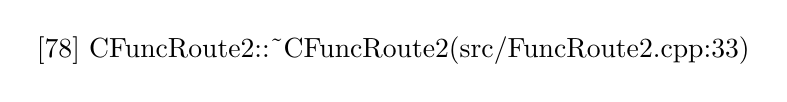
\begin{tikzpicture}[grow via three points={one child at (0.5,-0.7) and two children at (0.5,-0.7) and (0.5,-1.4)}, edge from parent path={(\tikzparentnode.south) |- (\tikzchildnode.west)}]
\node {[78] CFuncRoute2::\~{}CFuncRoute2(src/FuncRoute2.cpp:33)}
;
\end{tikzpicture}

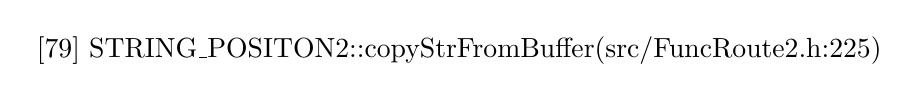
\begin{tikzpicture}[grow via three points={one child at (0.5,-0.7) and two children at (0.5,-0.7) and (0.5,-1.4)}, edge from parent path={(\tikzparentnode.south) |- (\tikzchildnode.west)}]
\node {[79] STRING\_POSITON2::copyStrFromBuffer(src/FuncRoute2.h:225)}
;
\end{tikzpicture}

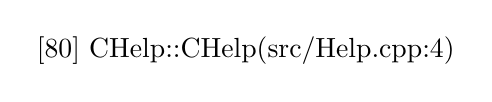
\begin{tikzpicture}[grow via three points={one child at (0.5,-0.7) and two children at (0.5,-0.7) and (0.5,-1.4)}, edge from parent path={(\tikzparentnode.south) |- (\tikzchildnode.west)}]
\node {[80] CHelp::CHelp(src/Help.cpp:4)}
;
\end{tikzpicture}

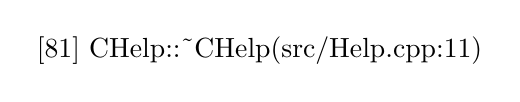
\begin{tikzpicture}[grow via three points={one child at (0.5,-0.7) and two children at (0.5,-0.7) and (0.5,-1.4)}, edge from parent path={(\tikzparentnode.south) |- (\tikzchildnode.west)}]
\node {[81] CHelp::\~{}CHelp(src/Help.cpp:11)}
;
\end{tikzpicture}

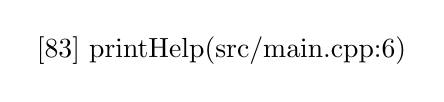
\begin{tikzpicture}[grow via three points={one child at (0.5,-0.7) and two children at (0.5,-0.7) and (0.5,-1.4)}, edge from parent path={(\tikzparentnode.south) |- (\tikzchildnode.west)}]
\node {[83] printHelp(src/main.cpp:6)}
;
\end{tikzpicture}

\begin{tikzpicture}[grow via three points={one child at (0.5,-0.7) and two children at (0.5,-0.7) and (0.5,-1.4)}, edge from parent path={(\tikzparentnode.south) |- (\tikzchildnode.west)}]
\node {[84] main(src/main.cpp:26)}
    child { node {[82] CHelp::printHelp(src/Help.cpp:18)} 
        }
    child { node {[18] CFuncRoute::splitDirsBySemicolon(src/FuncRoute.cpp:46)} 
        }
    child { node {[18] CFuncRoute::splitDirsBySemicolon(src/FuncRoute.cpp:46)} 
        }
    child { node {[19] CFuncRoute::findAllFunctionsName(src/FuncRoute.cpp:91)} 
        child { node {[171] get\_nested\_dir\_files(win32/shared\_library\_win32.cpp:135)} 
            child { node {[171] get\_nested\_dir\_files(win32/shared\_library\_win32.cpp:135)} 
                }
            }
            child [missing] {}
        child { node {[171] get\_nested\_dir\_files(win32/shared\_library\_win32.cpp:135)} 
            child { node {[171] get\_nested\_dir\_files(win32/shared\_library\_win32.cpp:135)} 
                }
            }
            child [missing] {}
        child { node {[31] CFuncRoute::findAllMacros(src/FuncRoute.cpp:1468)} 
            child { node {[25] CFuncRoute::replaceAllCodeCommentsBySpace(src/FuncRoute.cpp:1044)} 
                child { node {[26] CFuncRoute::findCurLineStartAndEndPos(src/FuncRoute.cpp:1149)} 
                    }
                child { node {[27] CFuncRoute::isBetweenInDoubleQuotes(src/FuncRoute.cpp:1191)} 
                    child { node {[43] CFuncRoute::findCharForward(src/FuncRoute.cpp:2682)} 
                        }
                    child { node {[43] CFuncRoute::findCharForward(src/FuncRoute.cpp:2682)} 
                        }
                    }
                    child [missing] {}
                    child [missing] {}
                child { node {[26] CFuncRoute::findCurLineStartAndEndPos(src/FuncRoute.cpp:1149)} 
                    }
                child { node {[27] CFuncRoute::isBetweenInDoubleQuotes(src/FuncRoute.cpp:1191)} 
                    child { node {[43] CFuncRoute::findCharForward(src/FuncRoute.cpp:2682)} 
                        }
                    child { node {[43] CFuncRoute::findCharForward(src/FuncRoute.cpp:2682)} 
                        }
                    }
                    child [missing] {}
                    child [missing] {}
                    }
                    child [missing] {}
                    child [missing] {}
                    child [missing] {}
                    child [missing] {}
                    child [missing] {}
                    child [missing] {}
                    child [missing] {}
                    child [missing] {}
                    }
                    child [missing] {}
                    child [missing] {}
                    child [missing] {}
                    child [missing] {}
                    child [missing] {}
                    child [missing] {}
                    child [missing] {}
                    child [missing] {}
                    child [missing] {}
        child { node {[21] CFuncRoute::search\_CPP\_FuncName(src/FuncRoute.cpp:266)} 
            child { node {[25] CFuncRoute::replaceAllCodeCommentsBySpace(src/FuncRoute.cpp:1044)} 
                child { node {[26] CFuncRoute::findCurLineStartAndEndPos(src/FuncRoute.cpp:1149)} 
                    }
                child { node {[27] CFuncRoute::isBetweenInDoubleQuotes(src/FuncRoute.cpp:1191)} 
                    child { node {[43] CFuncRoute::findCharForward(src/FuncRoute.cpp:2682)} 
                        }
                    child { node {[43] CFuncRoute::findCharForward(src/FuncRoute.cpp:2682)} 
                        }
                    }
                    child [missing] {}
                    child [missing] {}
                child { node {[26] CFuncRoute::findCurLineStartAndEndPos(src/FuncRoute.cpp:1149)} 
                    }
                child { node {[27] CFuncRoute::isBetweenInDoubleQuotes(src/FuncRoute.cpp:1191)} 
                    child { node {[43] CFuncRoute::findCharForward(src/FuncRoute.cpp:2682)} 
                        }
                    child { node {[43] CFuncRoute::findCharForward(src/FuncRoute.cpp:2682)} 
                        }
                    }
                    child [missing] {}
                    child [missing] {}
                    }
                    child [missing] {}
                    child [missing] {}
                    child [missing] {}
                    child [missing] {}
                    child [missing] {}
                    child [missing] {}
                    child [missing] {}
                    child [missing] {}
            child { node {[28] CFuncRoute::replaceAllStrBySpace(src/FuncRoute.cpp:1269)} 
                }
            child { node {[29] CFuncRoute::replaceAllMacroDefineStrBySpace(src/FuncRoute.cpp:1383)} 
                child { node {[38] CFuncRoute::skipWhiteSpaceForward(src/FuncRoute.cpp:2487)} 
                    }
                child { node {[43] CFuncRoute::findCharForward(src/FuncRoute.cpp:2682)} 
                    }
                }
                child [missing] {}
                child [missing] {}
            child { node {[32] CFuncRoute::findAllClassAndStructDeclare(src/FuncRoute.cpp:1709)} 
                child { node {[57] CFuncRoute::isValidVarChar(src/FuncRoute.cpp:3268)} 
                    }
                child { node {[58] CFuncRoute::isWhiteSpace(src/FuncRoute.cpp:3282)} 
                    }
                child { node {[38] CFuncRoute::skipWhiteSpaceForward(src/FuncRoute.cpp:2487)} 
                    }
                child { node {[49] CFuncRoute::findStrForward(src/FuncRoute.cpp:2875)} 
                    }
                child { node {[7] STRING\_POSITON::copyStrFromBuffer(src/CommonData.h:39)} 
                    }
                child { node {[43] CFuncRoute::findCharForward(src/FuncRoute.cpp:2682)} 
                    }
                child { node {[43] CFuncRoute::findCharForward(src/FuncRoute.cpp:2682)} 
                    }
                child { node {[60] CFuncRoute::statBufferLinesCount(src/FuncRoute.cpp:3338)} 
                    }
                child { node {[40] CFuncRoute::findPairCharForward(src/FuncRoute.cpp:2550)} 
                    }
                child { node {[60] CFuncRoute::statBufferLinesCount(src/FuncRoute.cpp:3338)} 
                    }
                child { node {[7] STRING\_POSITON::copyStrFromBuffer(src/CommonData.h:39)} 
                    }
                child { node {[43] CFuncRoute::findCharForward(src/FuncRoute.cpp:2682)} 
                    }
                child { node {[43] CFuncRoute::findCharForward(src/FuncRoute.cpp:2682)} 
                    }
                child { node {[38] CFuncRoute::skipWhiteSpaceForward(src/FuncRoute.cpp:2487)} 
                    }
                child { node {[39] CFuncRoute::skipWhiteSpaceBack(src/FuncRoute.cpp:2518)} 
                    }
                child { node {[7] STRING\_POSITON::copyStrFromBuffer(src/CommonData.h:39)} 
                    }
                child { node {[64] CFuncRoute::splitParentsClass(src/FuncRoute.cpp:3459)} 
                    }
                child { node {[43] CFuncRoute::findCharForward(src/FuncRoute.cpp:2682)} 
                    }
                child { node {[43] CFuncRoute::findCharForward(src/FuncRoute.cpp:2682)} 
                    }
                child { node {[38] CFuncRoute::skipWhiteSpaceForward(src/FuncRoute.cpp:2487)} 
                    }
                child { node {[49] CFuncRoute::findStrForward(src/FuncRoute.cpp:2875)} 
                    }
                child { node {[7] STRING\_POSITON::copyStrFromBuffer(src/CommonData.h:39)} 
                    }
                child { node {[65] CFuncRoute::findAllMemberVarsInClassDeclare(src/FuncRoute.cpp:3566)} 
                    child { node {[43] CFuncRoute::findCharForward(src/FuncRoute.cpp:2682)} 
                        }
                    child { node {[47] CFuncRoute::findCharBackStop(src/FuncRoute.cpp:2797)} 
                        }
                    child { node {[40] CFuncRoute::findPairCharForward(src/FuncRoute.cpp:2550)} 
                        }
                    child { node {[47] CFuncRoute::findCharBackStop(src/FuncRoute.cpp:2797)} 
                        }
                    child { node {[40] CFuncRoute::findPairCharForward(src/FuncRoute.cpp:2550)} 
                        }
                    child { node {[39] CFuncRoute::skipWhiteSpaceBack(src/FuncRoute.cpp:2518)} 
                        }
                    child { node {[60] CFuncRoute::statBufferLinesCount(src/FuncRoute.cpp:3338)} 
                        }
                    child { node {[41] CFuncRoute::findPairCharBack(src/FuncRoute.cpp:2591)} 
                        }
                    child { node {[50] CFuncRoute::findStrBack(src/FuncRoute.cpp:2913)} 
                        }
                    child { node {[7] STRING\_POSITON::copyStrFromBuffer(src/CommonData.h:39)} 
                        }
                    child { node {[39] CFuncRoute::skipWhiteSpaceBack(src/FuncRoute.cpp:2518)} 
                        }
                    child { node {[52] CFuncRoute::findStrCharsBackGreedy(src/FuncRoute.cpp:3042)} 
                        }
                    child { node {[60] CFuncRoute::statBufferLinesCount(src/FuncRoute.cpp:3338)} 
                        }
                    child { node {[46] CFuncRoute::findCharsBackGreedy(src/FuncRoute.cpp:2766)} 
                        }
                    child { node {[38] CFuncRoute::skipWhiteSpaceForward(src/FuncRoute.cpp:2487)} 
                        }
                    child { node {[60] CFuncRoute::statBufferLinesCount(src/FuncRoute.cpp:3338)} 
                        }
                    child { node {[7] STRING\_POSITON::copyStrFromBuffer(src/CommonData.h:39)} 
                        }
                    child { node {[59] CFuncRoute::replaceTwoMoreWhiteSpaceByOneSpace(src/FuncRoute.cpp:3296)} 
                        }
                    child { node {[43] CFuncRoute::findCharForward(src/FuncRoute.cpp:2682)} 
                        }
                    child { node {[43] CFuncRoute::findCharForward(src/FuncRoute.cpp:2682)} 
                        }
                    child { node {[43] CFuncRoute::findCharForward(src/FuncRoute.cpp:2682)} 
                        }
                    }
                    child [missing] {}
                    child [missing] {}
                    child [missing] {}
                    child [missing] {}
                    child [missing] {}
                    child [missing] {}
                    child [missing] {}
                    child [missing] {}
                    child [missing] {}
                    child [missing] {}
                    child [missing] {}
                    child [missing] {}
                    child [missing] {}
                    child [missing] {}
                    child [missing] {}
                    child [missing] {}
                    child [missing] {}
                    child [missing] {}
                    child [missing] {}
                    child [missing] {}
                    child [missing] {}
                child { node {[66] CFuncRoute::findAllMemberFuncsInClassDeclare(src/FuncRoute.cpp:3725)} 
                    child { node {[35] CFuncRoute::findWholeFuncDeclare(src/FuncRoute.cpp:2186)} 
                        child { node {[40] CFuncRoute::findPairCharForward(src/FuncRoute.cpp:2550)} 
                            }
                        child { node {[7] STRING\_POSITON::copyStrFromBuffer(src/CommonData.h:39)} 
                            }
                        child { node {[39] CFuncRoute::skipWhiteSpaceBack(src/FuncRoute.cpp:2518)} 
                            }
                        child { node {[41] CFuncRoute::findPairCharBack(src/FuncRoute.cpp:2591)} 
                            }
                        child { node {[50] CFuncRoute::findStrBack(src/FuncRoute.cpp:2913)} 
                            }
                        child { node {[7] STRING\_POSITON::copyStrFromBuffer(src/CommonData.h:39)} 
                            }
                        child { node {[22] CFuncRoute::isKeyword(src/FuncRoute.cpp:831)} 
                            }
                        child { node {[39] CFuncRoute::skipWhiteSpaceBack(src/FuncRoute.cpp:2518)} 
                            }
                        child { node {[41] CFuncRoute::findPairCharBack(src/FuncRoute.cpp:2591)} 
                            }
                        child { node {[50] CFuncRoute::findStrBack(src/FuncRoute.cpp:2913)} 
                            }
                        child { node {[50] CFuncRoute::findStrBack(src/FuncRoute.cpp:2913)} 
                            }
                        child { node {[7] STRING\_POSITON::copyStrFromBuffer(src/CommonData.h:39)} 
                            }
                        child { node {[59] CFuncRoute::replaceTwoMoreWhiteSpaceByOneSpace(src/FuncRoute.cpp:3296)} 
                            }
                        }
                        child [missing] {}
                        child [missing] {}
                        child [missing] {}
                        child [missing] {}
                        child [missing] {}
                        child [missing] {}
                        child [missing] {}
                        child [missing] {}
                        child [missing] {}
                        child [missing] {}
                        child [missing] {}
                        child [missing] {}
                        child [missing] {}
                    child { node {[40] CFuncRoute::findPairCharForward(src/FuncRoute.cpp:2550)} 
                        }
                    }
                    child [missing] {}
                    child [missing] {}
                    child [missing] {}
                    child [missing] {}
                    child [missing] {}
                    child [missing] {}
                    child [missing] {}
                    child [missing] {}
                    child [missing] {}
                    child [missing] {}
                    child [missing] {}
                    child [missing] {}
                    child [missing] {}
                    child [missing] {}
                    child [missing] {}
                    }
                    child [missing] {}
                    child [missing] {}
                    child [missing] {}
                    child [missing] {}
                    child [missing] {}
                    child [missing] {}
                    child [missing] {}
                    child [missing] {}
                    child [missing] {}
                    child [missing] {}
                    child [missing] {}
                    child [missing] {}
                    child [missing] {}
                    child [missing] {}
                    child [missing] {}
                    child [missing] {}
                    child [missing] {}
                    child [missing] {}
                    child [missing] {}
                    child [missing] {}
                    child [missing] {}
                    child [missing] {}
                    child [missing] {}
                    child [missing] {}
                    child [missing] {}
                    child [missing] {}
                    child [missing] {}
                    child [missing] {}
                    child [missing] {}
                    child [missing] {}
                    child [missing] {}
                    child [missing] {}
                    child [missing] {}
                    child [missing] {}
                    child [missing] {}
                    child [missing] {}
                    child [missing] {}
                    child [missing] {}
                    child [missing] {}
                    child [missing] {}
                    child [missing] {}
                    child [missing] {}
                    child [missing] {}
                    child [missing] {}
                    child [missing] {}
                    child [missing] {}
                    child [missing] {}
                    child [missing] {}
                    child [missing] {}
                    child [missing] {}
                    child [missing] {}
                    child [missing] {}
                    child [missing] {}
                    child [missing] {}
                    child [missing] {}
                    child [missing] {}
                    child [missing] {}
                    child [missing] {}
                    child [missing] {}
                    child [missing] {}
            child { node {[43] CFuncRoute::findCharForward(src/FuncRoute.cpp:2682)} 
                }
            child { node {[60] CFuncRoute::statBufferLinesCount(src/FuncRoute.cpp:3338)} 
                }
            child { node {[40] CFuncRoute::findPairCharForward(src/FuncRoute.cpp:2550)} 
                }
            child { node {[60] CFuncRoute::statBufferLinesCount(src/FuncRoute.cpp:3338)} 
                }
            child { node {[53] CFuncRoute::findQueryStrBackStop(src/FuncRoute.cpp:3082)} 
                }
            child { node {[44] CFuncRoute::findCharForwardStop(src/FuncRoute.cpp:2707)} 
                }
            child { node {[39] CFuncRoute::skipWhiteSpaceBack(src/FuncRoute.cpp:2518)} 
                }
            child { node {[48] CFuncRoute::findCharStrsBackStop(src/FuncRoute.cpp:2831)} 
                }
            child { node {[42] CFuncRoute::findPairCharBackStop(src/FuncRoute.cpp:2632)} 
                }
            child { node {[60] CFuncRoute::statBufferLinesCount(src/FuncRoute.cpp:3338)} 
                }
            child { node {[39] CFuncRoute::skipWhiteSpaceBack(src/FuncRoute.cpp:2518)} 
                }
            child { node {[50] CFuncRoute::findStrBack(src/FuncRoute.cpp:2913)} 
                }
            child { node {[24] CFuncRoute::findOverloadOperatorsBack(src/FuncRoute.cpp:930)} 
                child { node {[53] CFuncRoute::findQueryStrBackStop(src/FuncRoute.cpp:3082)} 
                    }
                child { node {[38] CFuncRoute::skipWhiteSpaceForward(src/FuncRoute.cpp:2487)} 
                    }
                }
                child [missing] {}
                child [missing] {}
            child { node {[39] CFuncRoute::skipWhiteSpaceBack(src/FuncRoute.cpp:2518)} 
                }
            child { node {[47] CFuncRoute::findCharBackStop(src/FuncRoute.cpp:2797)} 
                }
            child { node {[50] CFuncRoute::findStrBack(src/FuncRoute.cpp:2913)} 
                }
            child { node {[39] CFuncRoute::skipWhiteSpaceBack(src/FuncRoute.cpp:2518)} 
                }
            child { node {[22] CFuncRoute::isKeyword(src/FuncRoute.cpp:831)} 
                }
            child { node {[39] CFuncRoute::skipWhiteSpaceBack(src/FuncRoute.cpp:2518)} 
                }
            child { node {[50] CFuncRoute::findStrBack(src/FuncRoute.cpp:2913)} 
                }
            child { node {[22] CFuncRoute::isKeyword(src/FuncRoute.cpp:831)} 
                }
            child { node {[39] CFuncRoute::skipWhiteSpaceBack(src/FuncRoute.cpp:2518)} 
                }
            child { node {[39] CFuncRoute::skipWhiteSpaceBack(src/FuncRoute.cpp:2518)} 
                }
            child { node {[39] CFuncRoute::skipWhiteSpaceBack(src/FuncRoute.cpp:2518)} 
                }
            child { node {[51] CFuncRoute::findStrVarTypeBack(src/FuncRoute.cpp:2961)} 
                child { node {[50] CFuncRoute::findStrBack(src/FuncRoute.cpp:2913)} 
                    }
                child { node {[41] CFuncRoute::findPairCharBack(src/FuncRoute.cpp:2591)} 
                    }
                child { node {[39] CFuncRoute::skipWhiteSpaceBack(src/FuncRoute.cpp:2518)} 
                    }
                child { node {[50] CFuncRoute::findStrBack(src/FuncRoute.cpp:2913)} 
                    }
                }
                child [missing] {}
                child [missing] {}
                child [missing] {}
                child [missing] {}
            child { node {[39] CFuncRoute::skipWhiteSpaceBack(src/FuncRoute.cpp:2518)} 
                }
            child { node {[51] CFuncRoute::findStrVarTypeBack(src/FuncRoute.cpp:2961)} 
                child { node {[50] CFuncRoute::findStrBack(src/FuncRoute.cpp:2913)} 
                    }
                child { node {[41] CFuncRoute::findPairCharBack(src/FuncRoute.cpp:2591)} 
                    }
                child { node {[39] CFuncRoute::skipWhiteSpaceBack(src/FuncRoute.cpp:2518)} 
                    }
                child { node {[50] CFuncRoute::findStrBack(src/FuncRoute.cpp:2913)} 
                    }
                }
                child [missing] {}
                child [missing] {}
                child [missing] {}
                child [missing] {}
            child { node {[23] CFuncRoute::isKeywordVarType(src/FuncRoute.cpp:869)} 
                }
            child { node {[38] CFuncRoute::skipWhiteSpaceForward(src/FuncRoute.cpp:2487)} 
                }
            child { node {[7] STRING\_POSITON::copyStrFromBuffer(src/CommonData.h:39)} 
                }
            child { node {[7] STRING\_POSITON::copyStrFromBuffer(src/CommonData.h:39)} 
                }
            child { node {[7] STRING\_POSITON::copyStrFromBuffer(src/CommonData.h:39)} 
                }
            child { node {[7] STRING\_POSITON::copyStrFromBuffer(src/CommonData.h:39)} 
                }
            child { node {[7] STRING\_POSITON::copyStrFromBuffer(src/CommonData.h:39)} 
                }
            child { node {[7] STRING\_POSITON::copyStrFromBuffer(src/CommonData.h:39)} 
                }
            child { node {[33] CFuncRoute::findAllFuncsInFunctionBody(src/FuncRoute.cpp:1885)} 
                child { node {[34] CFuncRoute::findWholeFuncCalled(src/FuncRoute.cpp:1926)} 
                    child { node {[40] CFuncRoute::findPairCharForward(src/FuncRoute.cpp:2550)} 
                        }
                    child { node {[7] STRING\_POSITON::copyStrFromBuffer(src/CommonData.h:39)} 
                        }
                    child { node {[39] CFuncRoute::skipWhiteSpaceBack(src/FuncRoute.cpp:2518)} 
                        }
                    child { node {[42] CFuncRoute::findPairCharBackStop(src/FuncRoute.cpp:2632)} 
                        }
                    child { node {[50] CFuncRoute::findStrBack(src/FuncRoute.cpp:2913)} 
                        }
                    child { node {[7] STRING\_POSITON::copyStrFromBuffer(src/CommonData.h:39)} 
                        }
                    child { node {[22] CFuncRoute::isKeyword(src/FuncRoute.cpp:831)} 
                        }
                    child { node {[39] CFuncRoute::skipWhiteSpaceBack(src/FuncRoute.cpp:2518)} 
                        }
                    child { node {[42] CFuncRoute::findPairCharBackStop(src/FuncRoute.cpp:2632)} 
                        }
                    child { node {[39] CFuncRoute::skipWhiteSpaceBack(src/FuncRoute.cpp:2518)} 
                        }
                    child { node {[42] CFuncRoute::findPairCharBackStop(src/FuncRoute.cpp:2632)} 
                        }
                    child { node {[50] CFuncRoute::findStrBack(src/FuncRoute.cpp:2913)} 
                        }
                    child { node {[42] CFuncRoute::findPairCharBackStop(src/FuncRoute.cpp:2632)} 
                        }
                    child { node {[50] CFuncRoute::findStrBack(src/FuncRoute.cpp:2913)} 
                        }
                    child { node {[7] STRING\_POSITON::copyStrFromBuffer(src/CommonData.h:39)} 
                        }
                    child { node {[50] CFuncRoute::findStrBack(src/FuncRoute.cpp:2913)} 
                        }
                    child { node {[7] STRING\_POSITON::copyStrFromBuffer(src/CommonData.h:39)} 
                        }
                    child { node {[39] CFuncRoute::skipWhiteSpaceBack(src/FuncRoute.cpp:2518)} 
                        }
                    child { node {[39] CFuncRoute::skipWhiteSpaceBack(src/FuncRoute.cpp:2518)} 
                        }
                    child { node {[50] CFuncRoute::findStrBack(src/FuncRoute.cpp:2913)} 
                        }
                    child { node {[42] CFuncRoute::findPairCharBackStop(src/FuncRoute.cpp:2632)} 
                        }
                    child { node {[50] CFuncRoute::findStrBack(src/FuncRoute.cpp:2913)} 
                        }
                    child { node {[7] STRING\_POSITON::copyStrFromBuffer(src/CommonData.h:39)} 
                        }
                    child { node {[56] CFuncRoute::findVarDeclareBack(src/FuncRoute.cpp:3172)} 
                        child { node {[57] CFuncRoute::isValidVarChar(src/FuncRoute.cpp:3268)} 
                            }
                        child { node {[57] CFuncRoute::isValidVarChar(src/FuncRoute.cpp:3268)} 
                            }
                        child { node {[39] CFuncRoute::skipWhiteSpaceBack(src/FuncRoute.cpp:2518)} 
                            }
                        child { node {[39] CFuncRoute::skipWhiteSpaceBack(src/FuncRoute.cpp:2518)} 
                            }
                        child { node {[41] CFuncRoute::findPairCharBack(src/FuncRoute.cpp:2591)} 
                            }
                        child { node {[50] CFuncRoute::findStrBack(src/FuncRoute.cpp:2913)} 
                            }
                        child { node {[50] CFuncRoute::findStrBack(src/FuncRoute.cpp:2913)} 
                            }
                        child { node {[7] STRING\_POSITON::copyStrFromBuffer(src/CommonData.h:39)} 
                            }
                        child { node {[59] CFuncRoute::replaceTwoMoreWhiteSpaceByOneSpace(src/FuncRoute.cpp:3296)} 
                            }
                        }
                        child [missing] {}
                        child [missing] {}
                        child [missing] {}
                        child [missing] {}
                        child [missing] {}
                        child [missing] {}
                        child [missing] {}
                        child [missing] {}
                        child [missing] {}
                    child { node {[56] CFuncRoute::findVarDeclareBack(src/FuncRoute.cpp:3172)} 
                        child { node {[57] CFuncRoute::isValidVarChar(src/FuncRoute.cpp:3268)} 
                            }
                        child { node {[57] CFuncRoute::isValidVarChar(src/FuncRoute.cpp:3268)} 
                            }
                        child { node {[39] CFuncRoute::skipWhiteSpaceBack(src/FuncRoute.cpp:2518)} 
                            }
                        child { node {[39] CFuncRoute::skipWhiteSpaceBack(src/FuncRoute.cpp:2518)} 
                            }
                        child { node {[41] CFuncRoute::findPairCharBack(src/FuncRoute.cpp:2591)} 
                            }
                        child { node {[50] CFuncRoute::findStrBack(src/FuncRoute.cpp:2913)} 
                            }
                        child { node {[50] CFuncRoute::findStrBack(src/FuncRoute.cpp:2913)} 
                            }
                        child { node {[7] STRING\_POSITON::copyStrFromBuffer(src/CommonData.h:39)} 
                            }
                        child { node {[59] CFuncRoute::replaceTwoMoreWhiteSpaceByOneSpace(src/FuncRoute.cpp:3296)} 
                            }
                        }
                        child [missing] {}
                        child [missing] {}
                        child [missing] {}
                        child [missing] {}
                        child [missing] {}
                        child [missing] {}
                        child [missing] {}
                        child [missing] {}
                        child [missing] {}
                        }
                        child [missing] {}
                        child [missing] {}
                        child [missing] {}
                        child [missing] {}
                        child [missing] {}
                        child [missing] {}
                        child [missing] {}
                        child [missing] {}
                        child [missing] {}
                        child [missing] {}
                        child [missing] {}
                        child [missing] {}
                        child [missing] {}
                        child [missing] {}
                        child [missing] {}
                        child [missing] {}
                        child [missing] {}
                        child [missing] {}
                        child [missing] {}
                        child [missing] {}
                        child [missing] {}
                        child [missing] {}
                        child [missing] {}
                        child [missing] {}
                        child [missing] {}
                        child [missing] {}
                        child [missing] {}
                        child [missing] {}
                        child [missing] {}
                        child [missing] {}
                        child [missing] {}
                        child [missing] {}
                        child [missing] {}
                        child [missing] {}
                        child [missing] {}
                        child [missing] {}
                        child [missing] {}
                        child [missing] {}
                        child [missing] {}
                        child [missing] {}
                        child [missing] {}
                        child [missing] {}
                        child [missing] {}
                        }
                        child [missing] {}
                        child [missing] {}
                        child [missing] {}
                        child [missing] {}
                        child [missing] {}
                        child [missing] {}
                        child [missing] {}
                        child [missing] {}
                        child [missing] {}
                        child [missing] {}
                        child [missing] {}
                        child [missing] {}
                        child [missing] {}
                        child [missing] {}
                        child [missing] {}
                        child [missing] {}
                        child [missing] {}
                        child [missing] {}
                        child [missing] {}
                        child [missing] {}
                        child [missing] {}
                        child [missing] {}
                        child [missing] {}
                        child [missing] {}
                        child [missing] {}
                        child [missing] {}
                        child [missing] {}
                        child [missing] {}
                        child [missing] {}
                        child [missing] {}
                        child [missing] {}
                        child [missing] {}
                        child [missing] {}
                        child [missing] {}
                        child [missing] {}
                        child [missing] {}
                        child [missing] {}
                        child [missing] {}
                        child [missing] {}
                        child [missing] {}
                        child [missing] {}
                        child [missing] {}
                        child [missing] {}
                        child [missing] {}
                        }
                        child [missing] {}
                        child [missing] {}
                        child [missing] {}
                        child [missing] {}
                        child [missing] {}
                        child [missing] {}
                        child [missing] {}
                        child [missing] {}
                        child [missing] {}
                        child [missing] {}
                        child [missing] {}
                        child [missing] {}
                        child [missing] {}
                        child [missing] {}
                        child [missing] {}
                        child [missing] {}
                        child [missing] {}
                        child [missing] {}
                        child [missing] {}
                        child [missing] {}
                        child [missing] {}
                        child [missing] {}
                        child [missing] {}
                        child [missing] {}
                        child [missing] {}
                        child [missing] {}
                        child [missing] {}
                        child [missing] {}
                        child [missing] {}
                        child [missing] {}
                        child [missing] {}
                        child [missing] {}
                        child [missing] {}
                        child [missing] {}
                        child [missing] {}
                        child [missing] {}
                        child [missing] {}
                        child [missing] {}
                        child [missing] {}
                        child [missing] {}
                        child [missing] {}
                        child [missing] {}
                        child [missing] {}
                        child [missing] {}
                        child [missing] {}
                        child [missing] {}
                        child [missing] {}
                        child [missing] {}
                        child [missing] {}
                        child [missing] {}
                        child [missing] {}
                        child [missing] {}
                        child [missing] {}
                        child [missing] {}
                        child [missing] {}
                        child [missing] {}
                        child [missing] {}
                        child [missing] {}
                        child [missing] {}
                        child [missing] {}
                        child [missing] {}
                        child [missing] {}
                        child [missing] {}
                        child [missing] {}
                        child [missing] {}
                        child [missing] {}
                        child [missing] {}
                        child [missing] {}
                        child [missing] {}
                        child [missing] {}
                        child [missing] {}
                        child [missing] {}
                        child [missing] {}
                        child [missing] {}
                        child [missing] {}
                        child [missing] {}
                        child [missing] {}
                        child [missing] {}
                        child [missing] {}
                        child [missing] {}
                        child [missing] {}
                        child [missing] {}
                        child [missing] {}
                        child [missing] {}
                        child [missing] {}
                        child [missing] {}
                        child [missing] {}
                        child [missing] {}
                        child [missing] {}
                        child [missing] {}
                        child [missing] {}
                        child [missing] {}
                        child [missing] {}
                        child [missing] {}
                        child [missing] {}
                        child [missing] {}
                        child [missing] {}
                        child [missing] {}
                        child [missing] {}
                        child [missing] {}
                        child [missing] {}
                        child [missing] {}
                        child [missing] {}
                        child [missing] {}
                        child [missing] {}
                        child [missing] {}
                        child [missing] {}
                        child [missing] {}
                        child [missing] {}
                        child [missing] {}
                        child [missing] {}
                        child [missing] {}
                        child [missing] {}
                        child [missing] {}
                        child [missing] {}
                        child [missing] {}
                        child [missing] {}
                        child [missing] {}
                        child [missing] {}
                        child [missing] {}
                        child [missing] {}
                        child [missing] {}
                        child [missing] {}
                        child [missing] {}
                        child [missing] {}
                        child [missing] {}
                        child [missing] {}
                        child [missing] {}
                        child [missing] {}
                        child [missing] {}
                        child [missing] {}
                        child [missing] {}
                        child [missing] {}
                        child [missing] {}
                        child [missing] {}
                        child [missing] {}
                        child [missing] {}
                        child [missing] {}
                        child [missing] {}
                        child [missing] {}
                        child [missing] {}
                        child [missing] {}
                        child [missing] {}
                        child [missing] {}
                        child [missing] {}
                        child [missing] {}
                        child [missing] {}
                        child [missing] {}
                        child [missing] {}
                        child [missing] {}
                        child [missing] {}
                        child [missing] {}
                        child [missing] {}
                        child [missing] {}
                        child [missing] {}
                        child [missing] {}
                        child [missing] {}
                        child [missing] {}
                        child [missing] {}
                        child [missing] {}
                        child [missing] {}
                        child [missing] {}
                        child [missing] {}
                        child [missing] {}
        child { node {[68] CFuncRoute::statAllFuns(src/FuncRoute.cpp:3808)} 
            child { node {[63] CFuncRoute::updateParentClass(src/FuncRoute.cpp:3398)} 
                }
            child { node {[62] CFuncRoute::isParentClass(src/FuncRoute.cpp:3368)} 
                }
            child { node {[67] CFuncRoute::isFunctionArgsMatch(src/FuncRoute.cpp:3775)} 
                }
            child { node {[62] CFuncRoute::isParentClass(src/FuncRoute.cpp:3368)} 
                }
            child { node {[69] CFuncRoute::createAllFunsCalledTree(src/FuncRoute.cpp:4083)} 
                child { node {[70] CFuncRoute::createFunsCalledTree(src/FuncRoute.cpp:4177)} 
                    child { node {[71] CFuncRoute::getFuncsPos(src/FuncRoute.cpp:4239)} 
                        }
                    child { node {[71] CFuncRoute::getFuncsPos(src/FuncRoute.cpp:4239)} 
                        }
                    child { node {[70] CFuncRoute::createFunsCalledTree(src/FuncRoute.cpp:4177)} 
                        }
                    }
                    child [missing] {}
                    child [missing] {}
                    child [missing] {}
                child { node {[74] CFuncRoute::createPdfTexHeader(src/FuncRoute.cpp:4303)} 
                    }
                child { node {[75] CFuncRoute::createPdfTexLogo(src/FuncRoute.cpp:4319)} 
                    }
                child { node {[5] \_FUNC\_INDEX\_::printInfo(src/CommonData.cpp:87)} 
                    child { node {[3] \_FUNC\_INDEX\_::isRecursiveFunction(src/CommonData.cpp:22)} 
                        }
                    }
                    child [missing] {}
                    }
                    child [missing] {}
                    child [missing] {}
                    child [missing] {}
                    child [missing] {}
                    child [missing] {}
                    child [missing] {}
                    child [missing] {}
                    child [missing] {}
                    }
                    child [missing] {}
                    child [missing] {}
                    child [missing] {}
                    child [missing] {}
                    child [missing] {}
                    child [missing] {}
                    child [missing] {}
                    child [missing] {}
                    child [missing] {}
                    child [missing] {}
                    child [missing] {}
                    child [missing] {}
                    child [missing] {}
                    }
                    child [missing] {}
                    child [missing] {}
                    child [missing] {}
                    child [missing] {}
                    child [missing] {}
                    child [missing] {}
                    child [missing] {}
                    child [missing] {}
                    child [missing] {}
                    child [missing] {}
                    child [missing] {}
                    child [missing] {}
                    child [missing] {}
                    child [missing] {}
                    child [missing] {}
                    child [missing] {}
                    child [missing] {}
                    child [missing] {}
                    child [missing] {}
                    child [missing] {}
                    child [missing] {}
                    child [missing] {}
                    child [missing] {}
                    child [missing] {}
                    child [missing] {}
                    child [missing] {}
                    child [missing] {}
                    child [missing] {}
                    child [missing] {}
                    child [missing] {}
                    child [missing] {}
                    child [missing] {}
                    child [missing] {}
                    child [missing] {}
                    child [missing] {}
                    child [missing] {}
                    child [missing] {}
                    child [missing] {}
                    child [missing] {}
                    child [missing] {}
                    child [missing] {}
                    child [missing] {}
                    child [missing] {}
                    child [missing] {}
                    child [missing] {}
                    child [missing] {}
                    child [missing] {}
                    child [missing] {}
                    child [missing] {}
                    child [missing] {}
                    child [missing] {}
                    child [missing] {}
                    child [missing] {}
                    child [missing] {}
                    child [missing] {}
                    child [missing] {}
                    child [missing] {}
                    child [missing] {}
                    child [missing] {}
                    child [missing] {}
                    child [missing] {}
                    child [missing] {}
                    child [missing] {}
                    child [missing] {}
                    child [missing] {}
                    child [missing] {}
                    child [missing] {}
                    child [missing] {}
                    child [missing] {}
                    child [missing] {}
                    child [missing] {}
                    child [missing] {}
                    child [missing] {}
                    child [missing] {}
                    child [missing] {}
                    child [missing] {}
                    child [missing] {}
                    child [missing] {}
                    child [missing] {}
                    child [missing] {}
                    child [missing] {}
                    child [missing] {}
                    child [missing] {}
                    child [missing] {}
                    child [missing] {}
                    child [missing] {}
                    child [missing] {}
                    child [missing] {}
                    child [missing] {}
                    child [missing] {}
                    child [missing] {}
                    child [missing] {}
                    child [missing] {}
                    child [missing] {}
                    child [missing] {}
                    child [missing] {}
                    child [missing] {}
                    child [missing] {}
                    child [missing] {}
                    child [missing] {}
                    child [missing] {}
                    child [missing] {}
                    child [missing] {}
                    child [missing] {}
                    child [missing] {}
                    child [missing] {}
                    child [missing] {}
                    child [missing] {}
                    child [missing] {}
                    child [missing] {}
                    child [missing] {}
                    child [missing] {}
                    child [missing] {}
                    child [missing] {}
                    child [missing] {}
                    child [missing] {}
                    child [missing] {}
                    child [missing] {}
                    child [missing] {}
                    child [missing] {}
                    child [missing] {}
                    child [missing] {}
                    child [missing] {}
                    child [missing] {}
                    child [missing] {}
                    child [missing] {}
                    child [missing] {}
                    child [missing] {}
                    child [missing] {}
                    child [missing] {}
                    child [missing] {}
                    child [missing] {}
                    child [missing] {}
                    child [missing] {}
                    child [missing] {}
                    child [missing] {}
                    child [missing] {}
                    child [missing] {}
                    child [missing] {}
                    child [missing] {}
                    child [missing] {}
                    child [missing] {}
                    child [missing] {}
                    child [missing] {}
                    child [missing] {}
                    child [missing] {}
                    child [missing] {}
                    child [missing] {}
                    child [missing] {}
                    child [missing] {}
                    child [missing] {}
                    child [missing] {}
                    child [missing] {}
                    child [missing] {}
                    child [missing] {}
                    child [missing] {}
                    child [missing] {}
                    child [missing] {}
                    child [missing] {}
                    child [missing] {}
                    child [missing] {}
                    child [missing] {}
                    child [missing] {}
                    child [missing] {}
                    child [missing] {}
                    child [missing] {}
                    child [missing] {}
                    child [missing] {}
                    child [missing] {}
                    child [missing] {}
                    child [missing] {}
                    child [missing] {}
                    child [missing] {}
                    child [missing] {}
                    child [missing] {}
                    child [missing] {}
                    child [missing] {}
                    child [missing] {}
                    child [missing] {}
                    child [missing] {}
                    child [missing] {}
                    child [missing] {}
                    child [missing] {}
                    child [missing] {}
                    child [missing] {}
                    child [missing] {}
                    child [missing] {}
                    child [missing] {}
                    child [missing] {}
                    child [missing] {}
                    child [missing] {}
                    child [missing] {}
                    child [missing] {}
;
\end{tikzpicture}

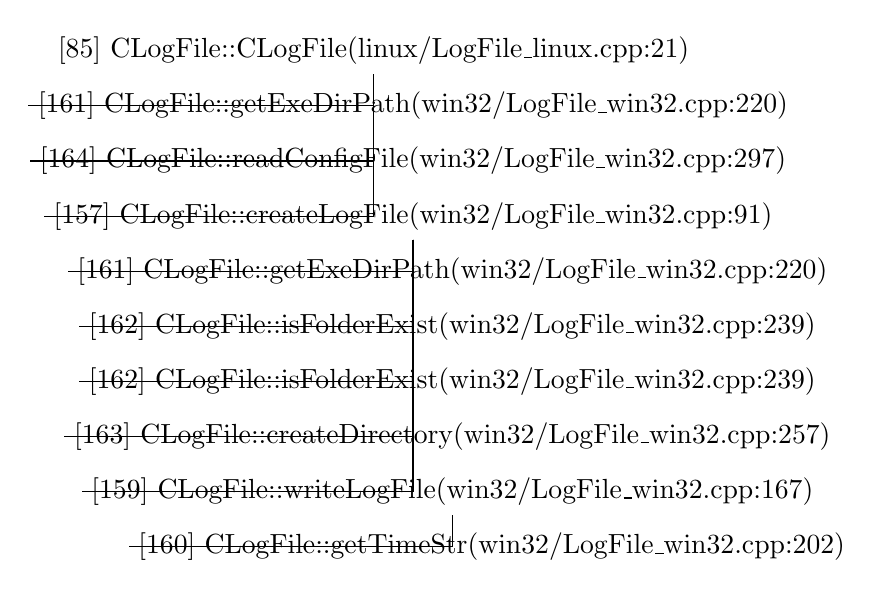
\begin{tikzpicture}[grow via three points={one child at (0.5,-0.7) and two children at (0.5,-0.7) and (0.5,-1.4)}, edge from parent path={(\tikzparentnode.south) |- (\tikzchildnode.west)}]
\node {[85] CLogFile::CLogFile(linux/LogFile\_linux.cpp:21)}
    child { node {[161] CLogFile::getExeDirPath(win32/LogFile\_win32.cpp:220)} 
        }
    child { node {[164] CLogFile::readConfigFile(win32/LogFile\_win32.cpp:297)} 
        }
    child { node {[157] CLogFile::createLogFile(win32/LogFile\_win32.cpp:91)} 
        child { node {[161] CLogFile::getExeDirPath(win32/LogFile\_win32.cpp:220)} 
            }
        child { node {[162] CLogFile::isFolderExist(win32/LogFile\_win32.cpp:239)} 
            }
        child { node {[162] CLogFile::isFolderExist(win32/LogFile\_win32.cpp:239)} 
            }
        child { node {[163] CLogFile::createDirectory(win32/LogFile\_win32.cpp:257)} 
            }
        child { node {[159] CLogFile::writeLogFile(win32/LogFile\_win32.cpp:167)} 
            child { node {[160] CLogFile::getTimeStr(win32/LogFile\_win32.cpp:202)} 
                }
            }
            child [missing] {}
            }
            child [missing] {}
            child [missing] {}
            child [missing] {}
            child [missing] {}
            child [missing] {}
            child [missing] {}
;
\end{tikzpicture}

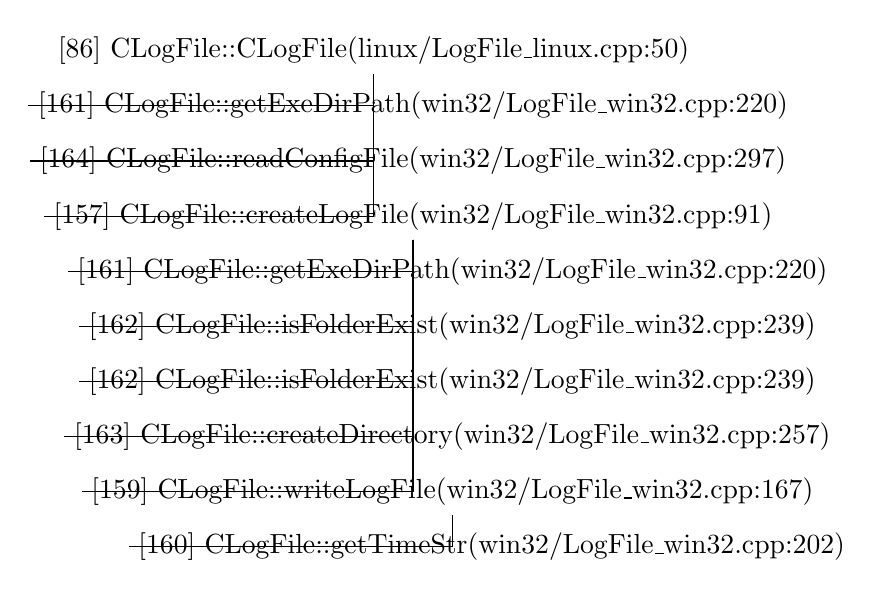
\begin{tikzpicture}[grow via three points={one child at (0.5,-0.7) and two children at (0.5,-0.7) and (0.5,-1.4)}, edge from parent path={(\tikzparentnode.south) |- (\tikzchildnode.west)}]
\node {[86] CLogFile::CLogFile(linux/LogFile\_linux.cpp:50)}
    child { node {[161] CLogFile::getExeDirPath(win32/LogFile\_win32.cpp:220)} 
        }
    child { node {[164] CLogFile::readConfigFile(win32/LogFile\_win32.cpp:297)} 
        }
    child { node {[157] CLogFile::createLogFile(win32/LogFile\_win32.cpp:91)} 
        child { node {[161] CLogFile::getExeDirPath(win32/LogFile\_win32.cpp:220)} 
            }
        child { node {[162] CLogFile::isFolderExist(win32/LogFile\_win32.cpp:239)} 
            }
        child { node {[162] CLogFile::isFolderExist(win32/LogFile\_win32.cpp:239)} 
            }
        child { node {[163] CLogFile::createDirectory(win32/LogFile\_win32.cpp:257)} 
            }
        child { node {[159] CLogFile::writeLogFile(win32/LogFile\_win32.cpp:167)} 
            child { node {[160] CLogFile::getTimeStr(win32/LogFile\_win32.cpp:202)} 
                }
            }
            child [missing] {}
            }
            child [missing] {}
            child [missing] {}
            child [missing] {}
            child [missing] {}
            child [missing] {}
            child [missing] {}
;
\end{tikzpicture}

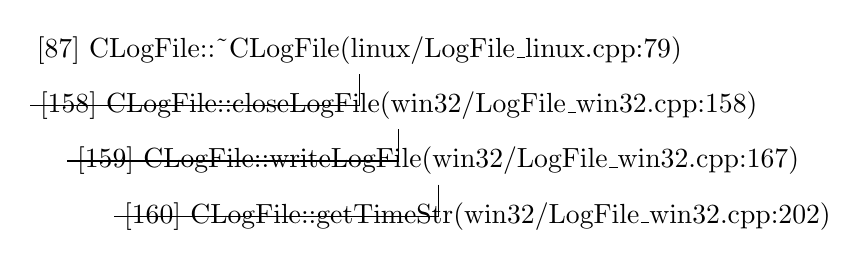
\begin{tikzpicture}[grow via three points={one child at (0.5,-0.7) and two children at (0.5,-0.7) and (0.5,-1.4)}, edge from parent path={(\tikzparentnode.south) |- (\tikzchildnode.west)}]
\node {[87] CLogFile::\~{}CLogFile(linux/LogFile\_linux.cpp:79)}
    child { node {[158] CLogFile::closeLogFile(win32/LogFile\_win32.cpp:158)} 
        child { node {[159] CLogFile::writeLogFile(win32/LogFile\_win32.cpp:167)} 
            child { node {[160] CLogFile::getTimeStr(win32/LogFile\_win32.cpp:202)} 
                }
            }
            child [missing] {}
            }
            child [missing] {}
            child [missing] {}
;
\end{tikzpicture}

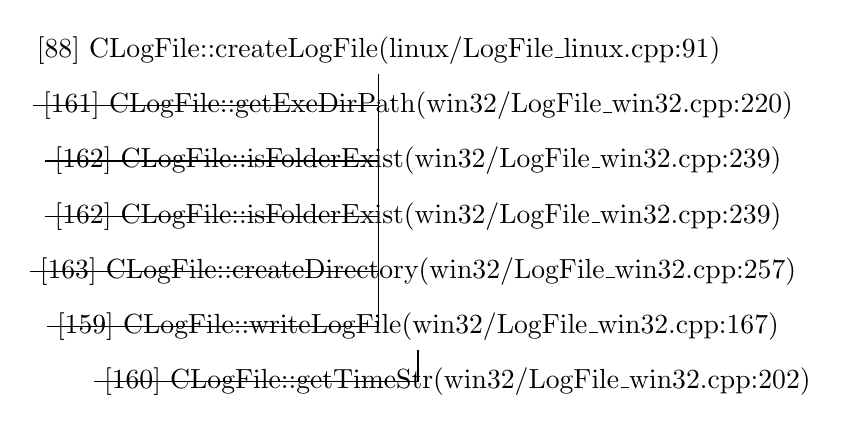
\begin{tikzpicture}[grow via three points={one child at (0.5,-0.7) and two children at (0.5,-0.7) and (0.5,-1.4)}, edge from parent path={(\tikzparentnode.south) |- (\tikzchildnode.west)}]
\node {[88] CLogFile::createLogFile(linux/LogFile\_linux.cpp:91)}
    child { node {[161] CLogFile::getExeDirPath(win32/LogFile\_win32.cpp:220)} 
        }
    child { node {[162] CLogFile::isFolderExist(win32/LogFile\_win32.cpp:239)} 
        }
    child { node {[162] CLogFile::isFolderExist(win32/LogFile\_win32.cpp:239)} 
        }
    child { node {[163] CLogFile::createDirectory(win32/LogFile\_win32.cpp:257)} 
        }
    child { node {[159] CLogFile::writeLogFile(win32/LogFile\_win32.cpp:167)} 
        child { node {[160] CLogFile::getTimeStr(win32/LogFile\_win32.cpp:202)} 
            }
        }
        child [missing] {}
;
\end{tikzpicture}

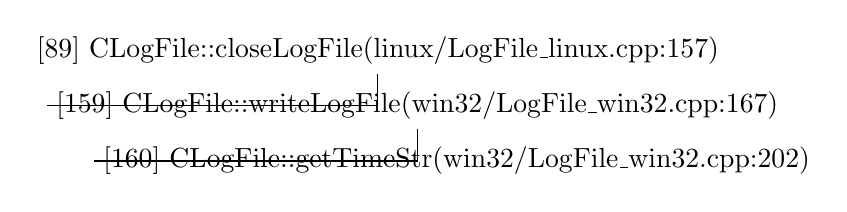
\begin{tikzpicture}[grow via three points={one child at (0.5,-0.7) and two children at (0.5,-0.7) and (0.5,-1.4)}, edge from parent path={(\tikzparentnode.south) |- (\tikzchildnode.west)}]
\node {[89] CLogFile::closeLogFile(linux/LogFile\_linux.cpp:157)}
    child { node {[159] CLogFile::writeLogFile(win32/LogFile\_win32.cpp:167)} 
        child { node {[160] CLogFile::getTimeStr(win32/LogFile\_win32.cpp:202)} 
            }
        }
        child [missing] {}
;
\end{tikzpicture}

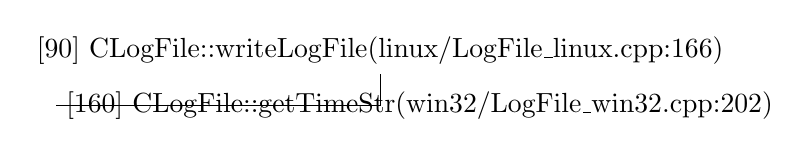
\begin{tikzpicture}[grow via three points={one child at (0.5,-0.7) and two children at (0.5,-0.7) and (0.5,-1.4)}, edge from parent path={(\tikzparentnode.south) |- (\tikzchildnode.west)}]
\node {[90] CLogFile::writeLogFile(linux/LogFile\_linux.cpp:166)}
    child { node {[160] CLogFile::getTimeStr(win32/LogFile\_win32.cpp:202)} 
        }
;
\end{tikzpicture}

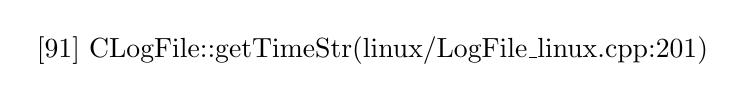
\begin{tikzpicture}[grow via three points={one child at (0.5,-0.7) and two children at (0.5,-0.7) and (0.5,-1.4)}, edge from parent path={(\tikzparentnode.south) |- (\tikzchildnode.west)}]
\node {[91] CLogFile::getTimeStr(linux/LogFile\_linux.cpp:201)}
;
\end{tikzpicture}

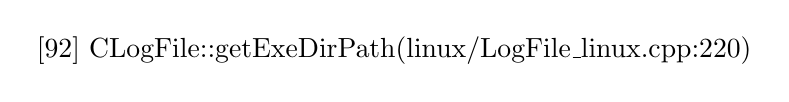
\begin{tikzpicture}[grow via three points={one child at (0.5,-0.7) and two children at (0.5,-0.7) and (0.5,-1.4)}, edge from parent path={(\tikzparentnode.south) |- (\tikzchildnode.west)}]
\node {[92] CLogFile::getExeDirPath(linux/LogFile\_linux.cpp:220)}
;
\end{tikzpicture}

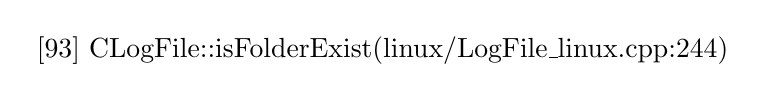
\begin{tikzpicture}[grow via three points={one child at (0.5,-0.7) and two children at (0.5,-0.7) and (0.5,-1.4)}, edge from parent path={(\tikzparentnode.south) |- (\tikzchildnode.west)}]
\node {[93] CLogFile::isFolderExist(linux/LogFile\_linux.cpp:244)}
;
\end{tikzpicture}

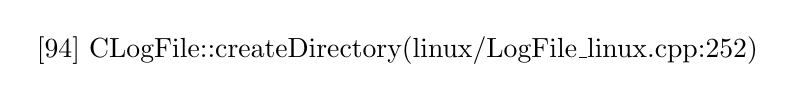
\begin{tikzpicture}[grow via three points={one child at (0.5,-0.7) and two children at (0.5,-0.7) and (0.5,-1.4)}, edge from parent path={(\tikzparentnode.south) |- (\tikzchildnode.west)}]
\node {[94] CLogFile::createDirectory(linux/LogFile\_linux.cpp:252)}
;
\end{tikzpicture}

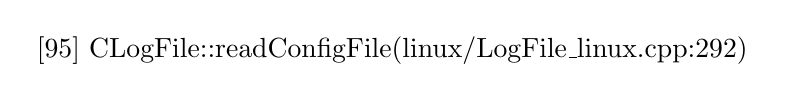
\begin{tikzpicture}[grow via three points={one child at (0.5,-0.7) and two children at (0.5,-0.7) and (0.5,-1.4)}, edge from parent path={(\tikzparentnode.south) |- (\tikzchildnode.west)}]
\node {[95] CLogFile::readConfigFile(linux/LogFile\_linux.cpp:292)}
;
\end{tikzpicture}

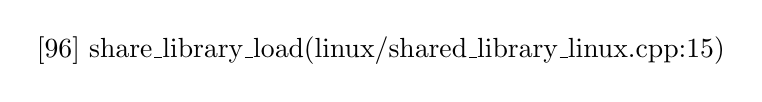
\begin{tikzpicture}[grow via three points={one child at (0.5,-0.7) and two children at (0.5,-0.7) and (0.5,-1.4)}, edge from parent path={(\tikzparentnode.south) |- (\tikzchildnode.west)}]
\node {[96] share\_library\_load(linux/shared\_library\_linux.cpp:15)}
;
\end{tikzpicture}

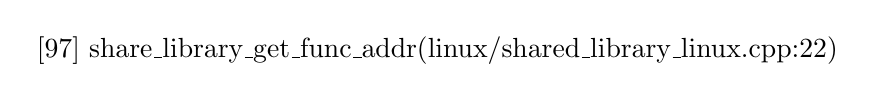
\begin{tikzpicture}[grow via three points={one child at (0.5,-0.7) and two children at (0.5,-0.7) and (0.5,-1.4)}, edge from parent path={(\tikzparentnode.south) |- (\tikzchildnode.west)}]
\node {[97] share\_library\_get\_func\_addr(linux/shared\_library\_linux.cpp:22)}
;
\end{tikzpicture}

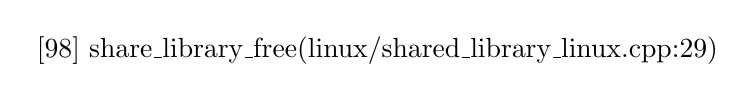
\begin{tikzpicture}[grow via three points={one child at (0.5,-0.7) and two children at (0.5,-0.7) and (0.5,-1.4)}, edge from parent path={(\tikzparentnode.south) |- (\tikzchildnode.west)}]
\node {[98] share\_library\_free(linux/shared\_library\_linux.cpp:29)}
;
\end{tikzpicture}

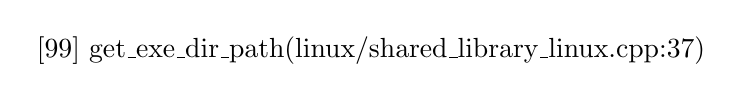
\begin{tikzpicture}[grow via three points={one child at (0.5,-0.7) and two children at (0.5,-0.7) and (0.5,-1.4)}, edge from parent path={(\tikzparentnode.south) |- (\tikzchildnode.west)}]
\node {[99] get\_exe\_dir\_path(linux/shared\_library\_linux.cpp:37)}
;
\end{tikzpicture}


\begin{tikzpicture}[grow via three points={one child at (0.5,-0.7) and two children at (0.5,-0.7) and (0.5,-1.4)}, edge from parent path={(\tikzparentnode.south) |- (\tikzchildnode.west)}]
\node {[100] get\_children\_dir\_name(linux/shared\_library\_linux.cpp:61)}
;
\end{tikzpicture}

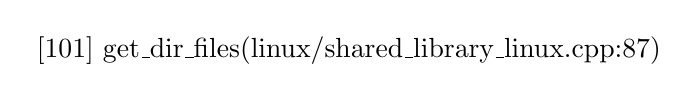
\begin{tikzpicture}[grow via three points={one child at (0.5,-0.7) and two children at (0.5,-0.7) and (0.5,-1.4)}, edge from parent path={(\tikzparentnode.south) |- (\tikzchildnode.west)}]
\node {[101] get\_dir\_files(linux/shared\_library\_linux.cpp:87)}
;
\end{tikzpicture}

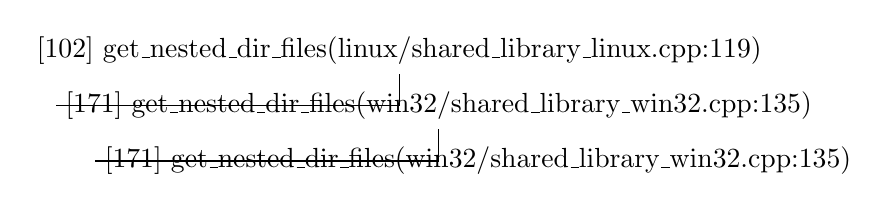
\begin{tikzpicture}[grow via three points={one child at (0.5,-0.7) and two children at (0.5,-0.7) and (0.5,-1.4)}, edge from parent path={(\tikzparentnode.south) |- (\tikzchildnode.west)}]
\node {[102] get\_nested\_dir\_files(linux/shared\_library\_linux.cpp:119)}
    child { node {[171] get\_nested\_dir\_files(win32/shared\_library\_win32.cpp:135)} 
        child { node {[171] get\_nested\_dir\_files(win32/shared\_library\_win32.cpp:135)} 
            }
        }
        child [missing] {}
;
\end{tikzpicture}

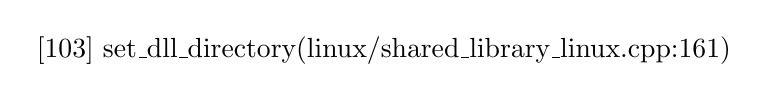
\begin{tikzpicture}[grow via three points={one child at (0.5,-0.7) and two children at (0.5,-0.7) and (0.5,-1.4)}, edge from parent path={(\tikzparentnode.south) |- (\tikzchildnode.west)}]
\node {[103] set\_dll\_directory(linux/shared\_library\_linux.cpp:161)}
;
\end{tikzpicture}

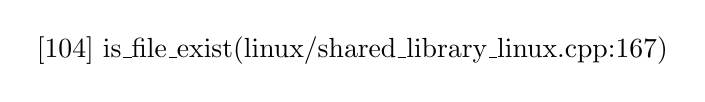
\begin{tikzpicture}[grow via three points={one child at (0.5,-0.7) and two children at (0.5,-0.7) and (0.5,-1.4)}, edge from parent path={(\tikzparentnode.south) |- (\tikzchildnode.west)}]
\node {[104] is\_file\_exist(linux/shared\_library\_linux.cpp:167)}
;
\end{tikzpicture}

\begin{tikzpicture}[grow via three points={one child at (0.5,-0.7) and two children at (0.5,-0.7) and (0.5,-1.4)}, edge from parent path={(\tikzparentnode.south) |- (\tikzchildnode.west)}]
\node {[105] print\_mem\_usage(linux/shared\_library\_linux.cpp:207)}
;
\end{tikzpicture}

\begin{tikzpicture}[grow via three points={one child at (0.5,-0.7) and two children at (0.5,-0.7) and (0.5,-1.4)}, edge from parent path={(\tikzparentnode.south) |- (\tikzchildnode.west)}]
\node {[106] print\_date\_time(linux/shared\_library\_linux.cpp:265)}
;
\end{tikzpicture}

\begin{tikzpicture}[grow via three points={one child at (0.5,-0.7) and two children at (0.5,-0.7) and (0.5,-1.4)}, edge from parent path={(\tikzparentnode.south) |- (\tikzchildnode.west)}]
\node {[107] gettid(linux/shared\_library\_linux.cpp:285)}
;
\end{tikzpicture}

\begin{tikzpicture}[grow via three points={one child at (0.5,-0.7) and two children at (0.5,-0.7) and (0.5,-1.4)}, edge from parent path={(\tikzparentnode.south) |- (\tikzchildnode.west)}]
\node {[108] get\_current\_thread\_id(linux/shared\_library\_linux.cpp:291)}
;
\end{tikzpicture}

\begin{tikzpicture}[grow via three points={one child at (0.5,-0.7) and two children at (0.5,-0.7) and (0.5,-1.4)}, edge from parent path={(\tikzparentnode.south) |- (\tikzchildnode.west)}]
\node {[109] create\_nested\_dir(linux/shared\_library\_linux.cpp:301)}
;
\end{tikzpicture}

\begin{tikzpicture}[grow via three points={one child at (0.5,-0.7) and two children at (0.5,-0.7) and (0.5,-1.4)}, edge from parent path={(\tikzparentnode.south) |- (\tikzchildnode.west)}]
\node {[110] CMutex::CMutex(linux/thread\_linux.cpp:11)}
;
\end{tikzpicture}

\begin{tikzpicture}[grow via three points={one child at (0.5,-0.7) and two children at (0.5,-0.7) and (0.5,-1.4)}, edge from parent path={(\tikzparentnode.south) |- (\tikzchildnode.west)}]
\node {[111] CMutex::\~{}CMutex(linux/thread\_linux.cpp:18)}
;
\end{tikzpicture}

\begin{tikzpicture}[grow via three points={one child at (0.5,-0.7) and two children at (0.5,-0.7) and (0.5,-1.4)}, edge from parent path={(\tikzparentnode.south) |- (\tikzchildnode.west)}]
\node {[112] CMutex::Lock(linux/thread\_linux.cpp:25)}
;
\end{tikzpicture}

\begin{tikzpicture}[grow via three points={one child at (0.5,-0.7) and two children at (0.5,-0.7) and (0.5,-1.4)}, edge from parent path={(\tikzparentnode.south) |- (\tikzchildnode.west)}]
\node {[113] CMutex::Unlock(linux/thread\_linux.cpp:31)}
;
\end{tikzpicture}

\begin{tikzpicture}[grow via three points={one child at (0.5,-0.7) and two children at (0.5,-0.7) and (0.5,-1.4)}, edge from parent path={(\tikzparentnode.south) |- (\tikzchildnode.west)}]
\node {[114] CMutex::Try(linux/thread\_linux.cpp:37)}
;
\end{tikzpicture}

\begin{tikzpicture}[grow via three points={one child at (0.5,-0.7) and two children at (0.5,-0.7) and (0.5,-1.4)}, edge from parent path={(\tikzparentnode.south) |- (\tikzchildnode.west)}]
\node {[115] CAutoMutex::CAutoMutex(linux/thread\_linux.cpp:44)}
;
\end{tikzpicture}

\begin{tikzpicture}[grow via three points={one child at (0.5,-0.7) and two children at (0.5,-0.7) and (0.5,-1.4)}, edge from parent path={(\tikzparentnode.south) |- (\tikzchildnode.west)}]
\node {[116] CAutoMutex::\~{}CAutoMutex(linux/thread\_linux.cpp:51)}
;
\end{tikzpicture}

\begin{tikzpicture}[grow via three points={one child at (0.5,-0.7) and two children at (0.5,-0.7) and (0.5,-1.4)}, edge from parent path={(\tikzparentnode.south) |- (\tikzchildnode.west)}]
\node {[117] CAutoMutex::Lock(linux/thread\_linux.cpp:57)}
;
\end{tikzpicture}

\begin{tikzpicture}[grow via three points={one child at (0.5,-0.7) and two children at (0.5,-0.7) and (0.5,-1.4)}, edge from parent path={(\tikzparentnode.south) |- (\tikzchildnode.west)}]
\node {[118] CAutoMutex::Unlock(linux/thread\_linux.cpp:72)}
;
\end{tikzpicture}

\begin{tikzpicture}[grow via three points={one child at (0.5,-0.7) and two children at (0.5,-0.7) and (0.5,-1.4)}, edge from parent path={(\tikzparentnode.south) |- (\tikzchildnode.west)}]
\node {[119] CSemaphore::CSemaphore(linux/thread\_linux.cpp:85)}
;
\end{tikzpicture}

\begin{tikzpicture}[grow via three points={one child at (0.5,-0.7) and two children at (0.5,-0.7) and (0.5,-1.4)}, edge from parent path={(\tikzparentnode.south) |- (\tikzchildnode.west)}]
\node {[120] CSemaphore::CSemaphore(linux/thread\_linux.cpp:91)}
;
\end{tikzpicture}

\begin{tikzpicture}[grow via three points={one child at (0.5,-0.7) and two children at (0.5,-0.7) and (0.5,-1.4)}, edge from parent path={(\tikzparentnode.south) |- (\tikzchildnode.west)}]
\node {[121] CSemaphore::\~{}CSemaphore(linux/thread\_linux.cpp:104)}
;
\end{tikzpicture}

\begin{tikzpicture}[grow via three points={one child at (0.5,-0.7) and two children at (0.5,-0.7) and (0.5,-1.4)}, edge from parent path={(\tikzparentnode.south) |- (\tikzchildnode.west)}]
\node {[122] CSemaphore::Post(linux/thread\_linux.cpp:111)}
;
\end{tikzpicture}

\begin{tikzpicture}[grow via three points={one child at (0.5,-0.7) and two children at (0.5,-0.7) and (0.5,-1.4)}, edge from parent path={(\tikzparentnode.south) |- (\tikzchildnode.west)}]
\node {[123] CSemaphore::Wait(linux/thread\_linux.cpp:124)}
;
\end{tikzpicture}

\begin{tikzpicture}[grow via three points={one child at (0.5,-0.7) and two children at (0.5,-0.7) and (0.5,-1.4)}, edge from parent path={(\tikzparentnode.south) |- (\tikzchildnode.west)}]
\node {[124] CEvent::CEvent(linux/thread\_linux.cpp:142)}
;
\end{tikzpicture}

\begin{tikzpicture}[grow via three points={one child at (0.5,-0.7) and two children at (0.5,-0.7) and (0.5,-1.4)}, edge from parent path={(\tikzparentnode.south) |- (\tikzchildnode.west)}]
\node {[125] CEvent::CEvent(linux/thread\_linux.cpp:148)}
;
\end{tikzpicture}

\begin{tikzpicture}[grow via three points={one child at (0.5,-0.7) and two children at (0.5,-0.7) and (0.5,-1.4)}, edge from parent path={(\tikzparentnode.south) |- (\tikzchildnode.west)}]
\node {[126] CEvent::\~{}CEvent(linux/thread\_linux.cpp:162)}
;
\end{tikzpicture}

\begin{tikzpicture}[grow via three points={one child at (0.5,-0.7) and two children at (0.5,-0.7) and (0.5,-1.4)}, edge from parent path={(\tikzparentnode.south) |- (\tikzchildnode.west)}]
\node {[127] CEvent::Init(linux/thread\_linux.cpp:170)}
;
\end{tikzpicture}

\begin{tikzpicture}[grow via three points={one child at (0.5,-0.7) and two children at (0.5,-0.7) and (0.5,-1.4)}, edge from parent path={(\tikzparentnode.south) |- (\tikzchildnode.west)}]
\node {[128] CEvent::Signal(linux/thread\_linux.cpp:187)}
;
\end{tikzpicture}

\begin{tikzpicture}[grow via three points={one child at (0.5,-0.7) and two children at (0.5,-0.7) and (0.5,-1.4)}, edge from parent path={(\tikzparentnode.south) |- (\tikzchildnode.west)}]
\node {[129] CEvent::Reset(linux/thread\_linux.cpp:210)}
;
\end{tikzpicture}

\begin{tikzpicture}[grow via three points={one child at (0.5,-0.7) and two children at (0.5,-0.7) and (0.5,-1.4)}, edge from parent path={(\tikzparentnode.south) |- (\tikzchildnode.west)}]
\node {[130] CEvent::Wait(linux/thread\_linux.cpp:222)}
;
\end{tikzpicture}

\begin{tikzpicture}[grow via three points={one child at (0.5,-0.7) and two children at (0.5,-0.7) and (0.5,-1.4)}, edge from parent path={(\tikzparentnode.south) |- (\tikzchildnode.west)}]
\node {[131] CEvent::TimedWait(linux/thread\_linux.cpp:236)}
;
\end{tikzpicture}

\begin{tikzpicture}[grow via three points={one child at (0.5,-0.7) and two children at (0.5,-0.7) and (0.5,-1.4)}, edge from parent path={(\tikzparentnode.south) |- (\tikzchildnode.west)}]
\node {[132] thread\_start(linux/thread\_linux.cpp:284)}
;
\end{tikzpicture}

\begin{tikzpicture}[grow via three points={one child at (0.5,-0.7) and two children at (0.5,-0.7) and (0.5,-1.4)}, edge from parent path={(\tikzparentnode.south) |- (\tikzchildnode.west)}]
\node {[133] CThread::CThread(linux/thread\_linux.cpp:298)}
;
\end{tikzpicture}

\begin{tikzpicture}[grow via three points={one child at (0.5,-0.7) and two children at (0.5,-0.7) and (0.5,-1.4)}, edge from parent path={(\tikzparentnode.south) |- (\tikzchildnode.west)}]
\node {[134] CThread::CThread(linux/thread\_linux.cpp:310)}
;
\end{tikzpicture}

\begin{tikzpicture}[grow via three points={one child at (0.5,-0.7) and two children at (0.5,-0.7) and (0.5,-1.4)}, edge from parent path={(\tikzparentnode.south) |- (\tikzchildnode.west)}]
\node {[135] CThread::\~{}CThread(linux/thread\_linux.cpp:322)}
;
\end{tikzpicture}

\begin{tikzpicture}[grow via three points={one child at (0.5,-0.7) and two children at (0.5,-0.7) and (0.5,-1.4)}, edge from parent path={(\tikzparentnode.south) |- (\tikzchildnode.west)}]
\node {[136] CThread::Begin(linux/thread\_linux.cpp:328)}
;
\end{tikzpicture}

\begin{tikzpicture}[grow via three points={one child at (0.5,-0.7) and two children at (0.5,-0.7) and (0.5,-1.4)}, edge from parent path={(\tikzparentnode.south) |- (\tikzchildnode.west)}]
\node {[137] CThread::End(linux/thread\_linux.cpp:345)}
;
\end{tikzpicture}

\begin{tikzpicture}[grow via three points={one child at (0.5,-0.7) and two children at (0.5,-0.7) and (0.5,-1.4)}, edge from parent path={(\tikzparentnode.south) |- (\tikzchildnode.west)}]
\node {[138] CThread::IsEnd(linux/thread\_linux.cpp:355)}
;
\end{tikzpicture}

\begin{tikzpicture}[grow via three points={one child at (0.5,-0.7) and two children at (0.5,-0.7) and (0.5,-1.4)}, edge from parent path={(\tikzparentnode.south) |- (\tikzchildnode.west)}]
\node {[139] CThread::Dead(linux/thread\_linux.cpp:367)}
;
\end{tikzpicture}

\begin{tikzpicture}[grow via three points={one child at (0.5,-0.7) and two children at (0.5,-0.7) and (0.5,-1.4)}, edge from parent path={(\tikzparentnode.south) |- (\tikzchildnode.west)}]
\node {[140] CThread::IsDead(linux/thread\_linux.cpp:374)}
;
\end{tikzpicture}

\begin{tikzpicture}[grow via three points={one child at (0.5,-0.7) and two children at (0.5,-0.7) and (0.5,-1.4)}, edge from parent path={(\tikzparentnode.south) |- (\tikzchildnode.west)}]
\node {[141] CThread::Wait(linux/thread\_linux.cpp:380)}
;
\end{tikzpicture}

\begin{tikzpicture}[grow via three points={one child at (0.5,-0.7) and two children at (0.5,-0.7) and (0.5,-1.4)}, edge from parent path={(\tikzparentnode.south) |- (\tikzchildnode.west)}]
\node {[142] CThread::TimedWait(linux/thread\_linux.cpp:387)}
;
\end{tikzpicture}

\begin{tikzpicture}[grow via three points={one child at (0.5,-0.7) and two children at (0.5,-0.7) and (0.5,-1.4)}, edge from parent path={(\tikzparentnode.south) |- (\tikzchildnode.west)}]
\node {[143] CThread::GetExitCode(linux/thread\_linux.cpp:401)}
;
\end{tikzpicture}

\begin{tikzpicture}[grow via three points={one child at (0.5,-0.7) and two children at (0.5,-0.7) and (0.5,-1.4)}, edge from parent path={(\tikzparentnode.south) |- (\tikzchildnode.west)}]
\node {[144] CThread::GetThreadId(linux/thread\_linux.cpp:409)}
;
\end{tikzpicture}

\begin{tikzpicture}[grow via three points={one child at (0.5,-0.7) and two children at (0.5,-0.7) and (0.5,-1.4)}, edge from parent path={(\tikzparentnode.south) |- (\tikzchildnode.west)}]
\node {[145] CThread::Suspend(linux/thread\_linux.cpp:415)}
;
\end{tikzpicture}

\begin{tikzpicture}[grow via three points={one child at (0.5,-0.7) and two children at (0.5,-0.7) and (0.5,-1.4)}, edge from parent path={(\tikzparentnode.south) |- (\tikzchildnode.west)}]
\node {[146] CThread::Resume(linux/thread\_linux.cpp:426)}
;
\end{tikzpicture}

\begin{tikzpicture}[grow via three points={one child at (0.5,-0.7) and two children at (0.5,-0.7) and (0.5,-1.4)}, edge from parent path={(\tikzparentnode.south) |- (\tikzchildnode.west)}]
\node {[147] CThread::IsSuspended(linux/thread\_linux.cpp:439)}
;
\end{tikzpicture}

\begin{tikzpicture}[grow via three points={one child at (0.5,-0.7) and two children at (0.5,-0.7) and (0.5,-1.4)}, edge from parent path={(\tikzparentnode.south) |- (\tikzchildnode.west)}]
\node {[149] atomic\_inc16(linux/thread\_linux.cpp:462)}
    child { node {[148] atomic\_add16(linux/thread\_linux.cpp:452)} 
        }
;
\end{tikzpicture}

\begin{tikzpicture}[grow via three points={one child at (0.5,-0.7) and two children at (0.5,-0.7) and (0.5,-1.4)}, edge from parent path={(\tikzparentnode.south) |- (\tikzchildnode.west)}]
\node {[150] atomic\_dec16(linux/thread\_linux.cpp:468)}
    child { node {[148] atomic\_add16(linux/thread\_linux.cpp:452)} 
        }
;
\end{tikzpicture}

\begin{tikzpicture}[grow via three points={one child at (0.5,-0.7) and two children at (0.5,-0.7) and (0.5,-1.4)}, edge from parent path={(\tikzparentnode.south) |- (\tikzchildnode.west)}]
\node {[151] time\_get\_tick(linux/timer\_linux.cpp:8)}
;
\end{tikzpicture}

\begin{tikzpicture}[grow via three points={one child at (0.5,-0.7) and two children at (0.5,-0.7) and (0.5,-1.4)}, edge from parent path={(\tikzparentnode.south) |- (\tikzchildnode.west)}]
\node {[152] time\_get\_frequency(linux/timer\_linux.cpp:17)}
;
\end{tikzpicture}

\begin{tikzpicture}[grow via three points={one child at (0.5,-0.7) and two children at (0.5,-0.7) and (0.5,-1.4)}, edge from parent path={(\tikzparentnode.south) |- (\tikzchildnode.west)}]
\node {[153] rdtsc(linux/timer\_linux.cpp:23)}
;
\end{tikzpicture}

\begin{tikzpicture}[grow via three points={one child at (0.5,-0.7) and two children at (0.5,-0.7) and (0.5,-1.4)}, edge from parent path={(\tikzparentnode.south) |- (\tikzchildnode.west)}]
\node {[154] CLogFile::CLogFile(win32/LogFile\_win32.cpp:21)}
    child { node {[161] CLogFile::getExeDirPath(win32/LogFile\_win32.cpp:220)} 
        }
    child { node {[164] CLogFile::readConfigFile(win32/LogFile\_win32.cpp:297)} 
        }
    child { node {[157] CLogFile::createLogFile(win32/LogFile\_win32.cpp:91)} 
        child { node {[161] CLogFile::getExeDirPath(win32/LogFile\_win32.cpp:220)} 
            }
        child { node {[162] CLogFile::isFolderExist(win32/LogFile\_win32.cpp:239)} 
            }
        child { node {[162] CLogFile::isFolderExist(win32/LogFile\_win32.cpp:239)} 
            }
        child { node {[163] CLogFile::createDirectory(win32/LogFile\_win32.cpp:257)} 
            }
        child { node {[159] CLogFile::writeLogFile(win32/LogFile\_win32.cpp:167)} 
            child { node {[160] CLogFile::getTimeStr(win32/LogFile\_win32.cpp:202)} 
                }
            }
            child [missing] {}
            }
            child [missing] {}
            child [missing] {}
            child [missing] {}
            child [missing] {}
            child [missing] {}
            child [missing] {}
;
\end{tikzpicture}

\begin{tikzpicture}[grow via three points={one child at (0.5,-0.7) and two children at (0.5,-0.7) and (0.5,-1.4)}, edge from parent path={(\tikzparentnode.south) |- (\tikzchildnode.west)}]
\node {[155] CLogFile::CLogFile(win32/LogFile\_win32.cpp:50)}
    child { node {[161] CLogFile::getExeDirPath(win32/LogFile\_win32.cpp:220)} 
        }
    child { node {[164] CLogFile::readConfigFile(win32/LogFile\_win32.cpp:297)} 
        }
    child { node {[157] CLogFile::createLogFile(win32/LogFile\_win32.cpp:91)} 
        child { node {[161] CLogFile::getExeDirPath(win32/LogFile\_win32.cpp:220)} 
            }
        child { node {[162] CLogFile::isFolderExist(win32/LogFile\_win32.cpp:239)} 
            }
        child { node {[162] CLogFile::isFolderExist(win32/LogFile\_win32.cpp:239)} 
            }
        child { node {[163] CLogFile::createDirectory(win32/LogFile\_win32.cpp:257)} 
            }
        child { node {[159] CLogFile::writeLogFile(win32/LogFile\_win32.cpp:167)} 
            child { node {[160] CLogFile::getTimeStr(win32/LogFile\_win32.cpp:202)} 
                }
            }
            child [missing] {}
            }
            child [missing] {}
            child [missing] {}
            child [missing] {}
            child [missing] {}
            child [missing] {}
            child [missing] {}
;
\end{tikzpicture}

\begin{tikzpicture}[grow via three points={one child at (0.5,-0.7) and two children at (0.5,-0.7) and (0.5,-1.4)}, edge from parent path={(\tikzparentnode.south) |- (\tikzchildnode.west)}]
\node {[156] CLogFile::\~{}CLogFile(win32/LogFile\_win32.cpp:79)}
    child { node {[158] CLogFile::closeLogFile(win32/LogFile\_win32.cpp:158)} 
        child { node {[159] CLogFile::writeLogFile(win32/LogFile\_win32.cpp:167)} 
            child { node {[160] CLogFile::getTimeStr(win32/LogFile\_win32.cpp:202)} 
                }
            }
            child [missing] {}
            }
            child [missing] {}
            child [missing] {}
;
\end{tikzpicture}

\begin{tikzpicture}[grow via three points={one child at (0.5,-0.7) and two children at (0.5,-0.7) and (0.5,-1.4)}, edge from parent path={(\tikzparentnode.south) |- (\tikzchildnode.west)}]
\node {[165] share\_library\_load(win32/shared\_library\_win32.cpp:12)}
;
\end{tikzpicture}

\begin{tikzpicture}[grow via three points={one child at (0.5,-0.7) and two children at (0.5,-0.7) and (0.5,-1.4)}, edge from parent path={(\tikzparentnode.south) |- (\tikzchildnode.west)}]
\node {[166] share\_library\_get\_func\_addr(win32/shared\_library\_win32.cpp:19)}
;
\end{tikzpicture}

\begin{tikzpicture}[grow via three points={one child at (0.5,-0.7) and two children at (0.5,-0.7) and (0.5,-1.4)}, edge from parent path={(\tikzparentnode.south) |- (\tikzchildnode.west)}]
\node {[167] share\_library\_free(win32/shared\_library\_win32.cpp:26)}
;
\end{tikzpicture}

\begin{tikzpicture}[grow via three points={one child at (0.5,-0.7) and two children at (0.5,-0.7) and (0.5,-1.4)}, edge from parent path={(\tikzparentnode.south) |- (\tikzchildnode.west)}]
\node {[168] get\_exe\_dir\_path(win32/shared\_library\_win32.cpp:34)}
;
\end{tikzpicture}

\begin{tikzpicture}[grow via three points={one child at (0.5,-0.7) and two children at (0.5,-0.7) and (0.5,-1.4)}, edge from parent path={(\tikzparentnode.south) |- (\tikzchildnode.west)}]
\node {[169] get\_children\_dir\_name(win32/shared\_library\_win32.cpp:65)}
;
\end{tikzpicture}

\begin{tikzpicture}[grow via three points={one child at (0.5,-0.7) and two children at (0.5,-0.7) and (0.5,-1.4)}, edge from parent path={(\tikzparentnode.south) |- (\tikzchildnode.west)}]
\node {[170] get\_dir\_files(win32/shared\_library\_win32.cpp:98)}
;
\end{tikzpicture}

\begin{tikzpicture}[grow via three points={one child at (0.5,-0.7) and two children at (0.5,-0.7) and (0.5,-1.4)}, edge from parent path={(\tikzparentnode.south) |- (\tikzchildnode.west)}]
\node {[172] set\_dll\_directory(win32/shared\_library\_win32.cpp:179)}
;
\end{tikzpicture}

\begin{tikzpicture}[grow via three points={one child at (0.5,-0.7) and two children at (0.5,-0.7) and (0.5,-1.4)}, edge from parent path={(\tikzparentnode.south) |- (\tikzchildnode.west)}]
\node {[173] is\_file\_exist(win32/shared\_library\_win32.cpp:186)}
;
\end{tikzpicture}

\begin{tikzpicture}[grow via three points={one child at (0.5,-0.7) and two children at (0.5,-0.7) and (0.5,-1.4)}, edge from parent path={(\tikzparentnode.south) |- (\tikzchildnode.west)}]
\node {[174] print\_mem\_usage(win32/shared\_library\_win32.cpp:199)}
;
\end{tikzpicture}

\begin{tikzpicture}[grow via three points={one child at (0.5,-0.7) and two children at (0.5,-0.7) and (0.5,-1.4)}, edge from parent path={(\tikzparentnode.south) |- (\tikzchildnode.west)}]
\node {[175] print\_date\_time(win32/shared\_library\_win32.cpp:218)}
;
\end{tikzpicture}

\begin{tikzpicture}[grow via three points={one child at (0.5,-0.7) and two children at (0.5,-0.7) and (0.5,-1.4)}, edge from parent path={(\tikzparentnode.south) |- (\tikzchildnode.west)}]
\node {[176] get\_current\_thread\_id(win32/shared\_library\_win32.cpp:238)}
;
\end{tikzpicture}

\begin{tikzpicture}[grow via three points={one child at (0.5,-0.7) and two children at (0.5,-0.7) and (0.5,-1.4)}, edge from parent path={(\tikzparentnode.south) |- (\tikzchildnode.west)}]
\node {[177] create\_nested\_dir(win32/shared\_library\_win32.cpp:246)}
;
\end{tikzpicture}

\begin{tikzpicture}[grow via three points={one child at (0.5,-0.7) and two children at (0.5,-0.7) and (0.5,-1.4)}, edge from parent path={(\tikzparentnode.south) |- (\tikzchildnode.west)}]
\node {[178] CMutex::CMutex(win32/thread\_win32.cpp:9)}
;
\end{tikzpicture}

\begin{tikzpicture}[grow via three points={one child at (0.5,-0.7) and two children at (0.5,-0.7) and (0.5,-1.4)}, edge from parent path={(\tikzparentnode.south) |- (\tikzchildnode.west)}]
\node {[179] CMutex::\~{}CMutex(win32/thread\_win32.cpp:15)}
;
\end{tikzpicture}

\begin{tikzpicture}[grow via three points={one child at (0.5,-0.7) and two children at (0.5,-0.7) and (0.5,-1.4)}, edge from parent path={(\tikzparentnode.south) |- (\tikzchildnode.west)}]
\node {[180] CMutex::Lock(win32/thread\_win32.cpp:22)}
;
\end{tikzpicture}

\begin{tikzpicture}[grow via three points={one child at (0.5,-0.7) and two children at (0.5,-0.7) and (0.5,-1.4)}, edge from parent path={(\tikzparentnode.south) |- (\tikzchildnode.west)}]
\node {[181] CMutex::Unlock(win32/thread\_win32.cpp:29)}
;
\end{tikzpicture}

\begin{tikzpicture}[grow via three points={one child at (0.5,-0.7) and two children at (0.5,-0.7) and (0.5,-1.4)}, edge from parent path={(\tikzparentnode.south) |- (\tikzchildnode.west)}]
\node {[182] CMutex::Try(win32/thread\_win32.cpp:36)}
;
\end{tikzpicture}

\begin{tikzpicture}[grow via three points={one child at (0.5,-0.7) and two children at (0.5,-0.7) and (0.5,-1.4)}, edge from parent path={(\tikzparentnode.south) |- (\tikzchildnode.west)}]
\node {[183] CAutoMutex::CAutoMutex(win32/thread\_win32.cpp:43)}
;
\end{tikzpicture}

\begin{tikzpicture}[grow via three points={one child at (0.5,-0.7) and two children at (0.5,-0.7) and (0.5,-1.4)}, edge from parent path={(\tikzparentnode.south) |- (\tikzchildnode.west)}]
\node {[184] CAutoMutex::\~{}CAutoMutex(win32/thread\_win32.cpp:50)}
;
\end{tikzpicture}

\begin{tikzpicture}[grow via three points={one child at (0.5,-0.7) and two children at (0.5,-0.7) and (0.5,-1.4)}, edge from parent path={(\tikzparentnode.south) |- (\tikzchildnode.west)}]
\node {[185] CAutoMutex::Lock(win32/thread\_win32.cpp:56)}
;
\end{tikzpicture}

\begin{tikzpicture}[grow via three points={one child at (0.5,-0.7) and two children at (0.5,-0.7) and (0.5,-1.4)}, edge from parent path={(\tikzparentnode.south) |- (\tikzchildnode.west)}]
\node {[186] CAutoMutex::Unlock(win32/thread\_win32.cpp:71)}
;
\end{tikzpicture}

\begin{tikzpicture}[grow via three points={one child at (0.5,-0.7) and two children at (0.5,-0.7) and (0.5,-1.4)}, edge from parent path={(\tikzparentnode.south) |- (\tikzchildnode.west)}]
\node {[187] CSemaphore::CSemaphore(win32/thread\_win32.cpp:84)}
;
\end{tikzpicture}

\begin{tikzpicture}[grow via three points={one child at (0.5,-0.7) and two children at (0.5,-0.7) and (0.5,-1.4)}, edge from parent path={(\tikzparentnode.south) |- (\tikzchildnode.west)}]
\node {[188] CSemaphore::CSemaphore(win32/thread\_win32.cpp:90)}
;
\end{tikzpicture}

\begin{tikzpicture}[grow via three points={one child at (0.5,-0.7) and two children at (0.5,-0.7) and (0.5,-1.4)}, edge from parent path={(\tikzparentnode.south) |- (\tikzchildnode.west)}]
\node {[189] CSemaphore::\~{}CSemaphore(win32/thread\_win32.cpp:98)}
;
\end{tikzpicture}

\begin{tikzpicture}[grow via three points={one child at (0.5,-0.7) and two children at (0.5,-0.7) and (0.5,-1.4)}, edge from parent path={(\tikzparentnode.south) |- (\tikzchildnode.west)}]
\node {[190] CSemaphore::Post(win32/thread\_win32.cpp:104)}
;
\end{tikzpicture}

\begin{tikzpicture}[grow via three points={one child at (0.5,-0.7) and two children at (0.5,-0.7) and (0.5,-1.4)}, edge from parent path={(\tikzparentnode.south) |- (\tikzchildnode.west)}]
\node {[191] CSemaphore::Wait(win32/thread\_win32.cpp:110)}
;
\end{tikzpicture}

\begin{tikzpicture}[grow via three points={one child at (0.5,-0.7) and two children at (0.5,-0.7) and (0.5,-1.4)}, edge from parent path={(\tikzparentnode.south) |- (\tikzchildnode.west)}]
\node {[192] CEvent::CEvent(win32/thread\_win32.cpp:117)}
;
\end{tikzpicture}

\begin{tikzpicture}[grow via three points={one child at (0.5,-0.7) and two children at (0.5,-0.7) and (0.5,-1.4)}, edge from parent path={(\tikzparentnode.south) |- (\tikzchildnode.west)}]
\node {[193] CEvent::CEvent(win32/thread\_win32.cpp:123)}
;
\end{tikzpicture}

\begin{tikzpicture}[grow via three points={one child at (0.5,-0.7) and two children at (0.5,-0.7) and (0.5,-1.4)}, edge from parent path={(\tikzparentnode.south) |- (\tikzchildnode.west)}]
\node {[194] CEvent::\~{}CEvent(win32/thread\_win32.cpp:131)}
;
\end{tikzpicture}

\begin{tikzpicture}[grow via three points={one child at (0.5,-0.7) and two children at (0.5,-0.7) and (0.5,-1.4)}, edge from parent path={(\tikzparentnode.south) |- (\tikzchildnode.west)}]
\node {[195] CEvent::Init(win32/thread\_win32.cpp:142)}
;
\end{tikzpicture}

\begin{tikzpicture}[grow via three points={one child at (0.5,-0.7) and two children at (0.5,-0.7) and (0.5,-1.4)}, edge from parent path={(\tikzparentnode.south) |- (\tikzchildnode.west)}]
\node {[196] CEvent::Signal(win32/thread\_win32.cpp:149)}
;
\end{tikzpicture}

\begin{tikzpicture}[grow via three points={one child at (0.5,-0.7) and two children at (0.5,-0.7) and (0.5,-1.4)}, edge from parent path={(\tikzparentnode.south) |- (\tikzchildnode.west)}]
\node {[197] CEvent::Reset(win32/thread\_win32.cpp:155)}
;
\end{tikzpicture}

\begin{tikzpicture}[grow via three points={one child at (0.5,-0.7) and two children at (0.5,-0.7) and (0.5,-1.4)}, edge from parent path={(\tikzparentnode.south) |- (\tikzchildnode.west)}]
\node {[198] CEvent::Wait(win32/thread\_win32.cpp:161)}
;
\end{tikzpicture}

\begin{tikzpicture}[grow via three points={one child at (0.5,-0.7) and two children at (0.5,-0.7) and (0.5,-1.4)}, edge from parent path={(\tikzparentnode.south) |- (\tikzchildnode.west)}]
\node {[199] CEvent::TimedWait(win32/thread\_win32.cpp:167)}
;
\end{tikzpicture}

\begin{tikzpicture}[grow via three points={one child at (0.5,-0.7) and two children at (0.5,-0.7) and (0.5,-1.4)}, edge from parent path={(\tikzparentnode.south) |- (\tikzchildnode.west)}]
\node {[200] CThread::CThread(win32/thread\_win32.cpp:189)}
;
\end{tikzpicture}

\begin{tikzpicture}[grow via three points={one child at (0.5,-0.7) and two children at (0.5,-0.7) and (0.5,-1.4)}, edge from parent path={(\tikzparentnode.south) |- (\tikzchildnode.west)}]
\node {[201] CThread::CThread(win32/thread\_win32.cpp:199)}
;
\end{tikzpicture}

\begin{tikzpicture}[grow via three points={one child at (0.5,-0.7) and two children at (0.5,-0.7) and (0.5,-1.4)}, edge from parent path={(\tikzparentnode.south) |- (\tikzchildnode.west)}]
\node {[202] CThread::\~{}CThread(win32/thread\_win32.cpp:212)}
;
\end{tikzpicture}

\begin{tikzpicture}[grow via three points={one child at (0.5,-0.7) and two children at (0.5,-0.7) and (0.5,-1.4)}, edge from parent path={(\tikzparentnode.south) |- (\tikzchildnode.west)}]
\node {[203] CThread::Begin(win32/thread\_win32.cpp:222)}
;
\end{tikzpicture}

\begin{tikzpicture}[grow via three points={one child at (0.5,-0.7) and two children at (0.5,-0.7) and (0.5,-1.4)}, edge from parent path={(\tikzparentnode.south) |- (\tikzchildnode.west)}]
\node {[204] CThread::End(win32/thread\_win32.cpp:240)}
;
\end{tikzpicture}

\begin{tikzpicture}[grow via three points={one child at (0.5,-0.7) and two children at (0.5,-0.7) and (0.5,-1.4)}, edge from parent path={(\tikzparentnode.south) |- (\tikzchildnode.west)}]
\node {[205] CThread::IsEnd(win32/thread\_win32.cpp:250)}
;
\end{tikzpicture}

\begin{tikzpicture}[grow via three points={one child at (0.5,-0.7) and two children at (0.5,-0.7) and (0.5,-1.4)}, edge from parent path={(\tikzparentnode.south) |- (\tikzchildnode.west)}]
\node {[206] CThread::Dead(win32/thread\_win32.cpp:262)}
;
\end{tikzpicture}

\begin{tikzpicture}[grow via three points={one child at (0.5,-0.7) and two children at (0.5,-0.7) and (0.5,-1.4)}, edge from parent path={(\tikzparentnode.south) |- (\tikzchildnode.west)}]
\node {[207] CThread::IsDead(win32/thread\_win32.cpp:269)}
;
\end{tikzpicture}

\begin{tikzpicture}[grow via three points={one child at (0.5,-0.7) and two children at (0.5,-0.7) and (0.5,-1.4)}, edge from parent path={(\tikzparentnode.south) |- (\tikzchildnode.west)}]
\node {[208] CThread::Wait(win32/thread\_win32.cpp:275)}
;
\end{tikzpicture}

\begin{tikzpicture}[grow via three points={one child at (0.5,-0.7) and two children at (0.5,-0.7) and (0.5,-1.4)}, edge from parent path={(\tikzparentnode.south) |- (\tikzchildnode.west)}]
\node {[209] CThread::TimedWait(win32/thread\_win32.cpp:281)}
;
\end{tikzpicture}

\begin{tikzpicture}[grow via three points={one child at (0.5,-0.7) and two children at (0.5,-0.7) and (0.5,-1.4)}, edge from parent path={(\tikzparentnode.south) |- (\tikzchildnode.west)}]
\node {[210] CThread::GetExitCode(win32/thread\_win32.cpp:303)}
;
\end{tikzpicture}

\begin{tikzpicture}[grow via three points={one child at (0.5,-0.7) and two children at (0.5,-0.7) and (0.5,-1.4)}, edge from parent path={(\tikzparentnode.south) |- (\tikzchildnode.west)}]
\node {[211] CThread::GetThreadId(win32/thread\_win32.cpp:326)}
;
\end{tikzpicture}

\begin{tikzpicture}[grow via three points={one child at (0.5,-0.7) and two children at (0.5,-0.7) and (0.5,-1.4)}, edge from parent path={(\tikzparentnode.south) |- (\tikzchildnode.west)}]
\node {[212] CThread::Suspend(win32/thread\_win32.cpp:332)}
;
\end{tikzpicture}

\begin{tikzpicture}[grow via three points={one child at (0.5,-0.7) and two children at (0.5,-0.7) and (0.5,-1.4)}, edge from parent path={(\tikzparentnode.south) |- (\tikzchildnode.west)}]
\node {[213] CThread::Resume(win32/thread\_win32.cpp:346)}
;
\end{tikzpicture}

\begin{tikzpicture}[grow via three points={one child at (0.5,-0.7) and two children at (0.5,-0.7) and (0.5,-1.4)}, edge from parent path={(\tikzparentnode.south) |- (\tikzchildnode.west)}]
\node {[214] CThread::IsSuspended(win32/thread\_win32.cpp:362)}
;
\end{tikzpicture}

\begin{tikzpicture}[grow via three points={one child at (0.5,-0.7) and two children at (0.5,-0.7) and (0.5,-1.4)}, edge from parent path={(\tikzparentnode.south) |- (\tikzchildnode.west)}]
\node {[215] atomic\_inc16(win32/thread\_win32.cpp:380)}
;
\end{tikzpicture}

\begin{tikzpicture}[grow via three points={one child at (0.5,-0.7) and two children at (0.5,-0.7) and (0.5,-1.4)}, edge from parent path={(\tikzparentnode.south) |- (\tikzchildnode.west)}]
\node {[216] atomic\_dec16(win32/thread\_win32.cpp:386)}
;
\end{tikzpicture}

\begin{tikzpicture}[grow via three points={one child at (0.5,-0.7) and two children at (0.5,-0.7) and (0.5,-1.4)}, edge from parent path={(\tikzparentnode.south) |- (\tikzchildnode.west)}]
\node {[217] time\_get\_tick(win32/timer\_win32.cpp:6)}
;
\end{tikzpicture}

\begin{tikzpicture}[grow via three points={one child at (0.5,-0.7) and two children at (0.5,-0.7) and (0.5,-1.4)}, edge from parent path={(\tikzparentnode.south) |- (\tikzchildnode.west)}]
\node {[218] time\_get\_frequency(win32/timer\_win32.cpp:15)}
;
\end{tikzpicture}

\begin{tikzpicture}[grow via three points={one child at (0.5,-0.7) and two children at (0.5,-0.7) and (0.5,-1.4)}, edge from parent path={(\tikzparentnode.south) |- (\tikzchildnode.west)}]
\node {[219] rdtsc(win32/timer\_win32.cpp:24)}
;
\end{tikzpicture}

\end{document}
